% !TEX program = xelatex
\documentclass[UTF8]{ctexart}
\usepackage{shumo}
\usepackage{amsmath,amssymb}
\usepackage{graphicx}
\usepackage{booktabs}
\usepackage{array}
\usepackage{float}
\usepackage{geometry}
\usepackage{url}
\geometry{a4paper,left=2.50cm,right=2.50cm,top=2.50cm,bottom=2.50cm}
\setcounter{tocdepth}{2}
\linespread{1.25}\selectfont
\setlength{\parindent}{2em}
\setlength{\parskip}{0pt}
\renewcommand{\contentsname}{目\quad 录}
\titlecontents{section}
  [0em]
  {\vspace{0.25em}\bfseries}
  {\contentslabel{2.2em}}
  {}
  {\titlerule*[0.6pc]{.}\contentspage}
\titlecontents{subsection}
  [2.2em]
  {\vspace{0.08em}}
  {\contentslabel{2.8em}}
  {}
  {\titlerule*[0.6pc]{.}\contentspage}

\title{\textbf{北极边缘冰区海冰演化与船舶安全航行建模}}
\author{}
\date{}

\newcommand{\dd}{\mathrm{d}}
\newcommand{\vect}[1]{\boldsymbol{#1}}
\lstset{
  breaklines=true,
  showstringspaces=false,
  basicstyle=\small\ttfamily,
  flexiblecolumns=true,
  keywordstyle=\color{blue},
  stringstyle=\color[rgb]{0.75,0,0.75},
  commentstyle=\songti\color[rgb]{0,0.5,0},
  tabsize=4
}

\begin{document}
\setcounter{page}{1}
\maketitle
\vspace{-0.95cm}

\renewcommand{\abstractname}{\sihao 摘\quad 要}
\begin{abstract}\xiaosihao
北极边缘冰区兼具海冰快速漂移、观测稀疏和航行风险随时间变化等特征。围绕海冰动力过程的合理简化、冰--水耦合正演、关键参数与初始场反演以及船舶航线决策，本文建立了一套由物理模型、数值算法和优化方法组成的递进式建模框架。

对于问题一，首先根据量纲一致性将海冰内力写为厚度加权应力通量散度 $\nabla\cdot(h_i\vect\sigma)$。在题定特征尺度下，惯性力与海冰科里奥利力的非负特征模长合计约占三项保留力特征模长合计的 $4.5636\%$，据此构造由 VP 内力、冰水拖曳力和风应力组成的瞬时三力平衡模型 M1。进一步设置完整模型及两个单删项模型进行对照：删除惯性对全过程速度较敏感，删除海冰科里奥利对速度方向和冰厚累积的影响更突出。收紧残差和减半时间步后，M1 相对 M0 的结构差异仍为 $7.78\%$--$13.44\%$，说明特征量级不能直接等同于场变量误差，M1 的适用范围需限定在缓变、非强剪切海况。

对于问题二，在 C 型交错网格上离散厚度加权 VP 算子，采用 Picard--GMRES/ILU 求解海冰非线性平衡，以 IMEX--Helmholtz 方法推进海水浅水方程，并用守恒迎风格式更新冰厚。时间预测、受保护 Anderson 加速和 ILU 复用使 $40\times20$ 网格 24 h 计算的墙钟中位数由 $504.787$ s 降至 $395.899$ s，优化前后时空场差异最大为 $0.0228\%$。在可完成的 $100\times50$ 替代网格上，24 h 区域平均冰厚为 $0.500000\ \mathrm m$，终时单元中心插值冰速最大值为 $0.208846\ \mathrm{m/s}$，冰体积保持至机器精度；题定 $200\times100$ 网格的 24 h 全时段计算尚未完成。

对于问题三，构造考虑固壁观测误差的加权最小二乘目标，分别采用粗--细网格搜索、Nelder--Mead 和差分进化反演 $(C_d,\alpha)$。网格搜索与差分进化在给定预算内均得到边界候选 $(0.015,0.5)$，目标函数值为 $636.2$；孪生试验能够恢复预设参数，表明真实观测下的较大残差主要反映模型--数据不一致，而非优化器完全失效。

对于问题四，以低频余弦基将初始冰厚场由 20000 个网格自由度降至 12 个谱系数，并采用带边界约束的 L-BFGS-B 求解背景正则化反问题。预算内候选使目标函数下降 $3.22\%$，最大厚度修正为 $0.0379\ \mathrm m$；以该场进行 48 h 正演，区域平均冰厚为 $0.484178\ \mathrm m$，最大冰速为 $0.107166\ \mathrm{m/s}$。

对于问题五，将逐小时冰密集度场嵌入时间分层路网。预报期内题设终点始终位于禁行区，故严格到达问题无可行解；对允许抵达最近可通行格的放宽问题，时变 Dijkstra 得到燃油 $0.484026\ \mathrm t$、航时 $0.6179\ \mathrm h$ 的候选路线，相比冻结 24 h 冰场的静态方案节油约 $0.13\%$。

研究结果表明，物理删项、数值加速、参数校准与航线优化应分别设置独立的验证标准；只有明确区分结构近似、离散误差和观测失配，才能使海冰预报结果可靠地服务于航行决策。

\textbf{关键词：}\quad 海冰动力学；瞬时三力平衡；黏塑性本构；冰水耦合；反问题；时变最短路
\end{abstract}

\pagestyle{plain}
\newpage
\linespread{1.25}\selectfont
\tableofcontents
\newpage

\section{绪论}

\subsection{研究背景与问题意义}

北极航线的商业价值日益凸显。相比传统苏伊士运河航线，北极东北航线具有缩短航程与降低燃料消耗的潜力；与此同时，偏远水域搜救能力有限、海冰快速演化和观测稀疏仍构成显著安全约束。Yan 等\cite{yan2026}对 2005--2024 年北方海航道事故的时空格局进行了系统分析，表明事故风险具有空间集聚与阶段变化特征。海冰范围减小并不等同于航行风险消失：边缘冰区的漂移、破碎和短时变化仍会改变可通行区域，因此有必要把海冰预报与航线决策置于同一建模链条中处理。

北极商船航行面临三个相互关联的难题：其一，海冰数值模式的关键参数（如冰水拖曳系数、风应力缩放系数）缺乏充分的现场约束，参数不确定性会直接传递到预报场；其二，有限观测难以约束全海域初始状态，从稀疏数据反演二维场本质上是病态问题；其三，高纬度通信和计算资源受限，冰情预报还需要及时转化为可执行的航线决策。这三个难题依次对应问题三、四、五：先校准模式参数，再估计初始冰厚场，最后将预报场转化为航行方案。因此，本文研究的不是孤立的数值求解器，而是一条“环境观测 $\to$ 状态估计 $\to$ 航行决策”的连续建模链条。

海冰动力模型大体可分为连续介质模型和离散单元模型。离散单元法能够描述冰块碰撞、旋转和破裂，适合小尺度碎冰动力过程，但其计算量随冰块数量快速增长，也难以与区域浅水方程和大尺度反演直接耦合；连续介质模型则把冰盖视为等效介质，便于在规则网格上同时求解速度、厚度和海水响应。Hibler 提出的黏塑性模型能够用统一的屈服曲线表示冰盖的挤压、剪切和近刚性运动，至今仍是大尺度海冰数值模式的重要基础\cite{hibler1979,feltham2008}。考虑到本题空间尺度为 $20\ \mathrm{km}\times10\ \mathrm{km}$、计算任务包含多次正演与反演，本文选择连续介质 VP 模型作为主框架，并把碎冰和裂隙区域列为适用边界，而不额外引入高成本的颗粒碰撞模型。

在数值层面，本题同时包含快速重力波、非线性 VP 流变和守恒输运三种不同性质的过程。若全部显式推进，题定 $300\ \mathrm s$ 时间步将远超浅水重力波的稳定上限；若全部采用大型单体隐式求解，又会使每次参数搜索的代价难以承受。本文因而采用分块耦合思路：海水快模态半隐式处理，海冰非线性平衡迭代求解，冰厚采用守恒格式更新，并通过外层固定点协调界面拖曳。该选择兼顾了物理可解释性、计算稳定性和后续反演对重复正演的需求。

\subsection{问题重述与任务分解}

本题以北极边缘冰区矩形海域 $[0,L_x]\times[0,L_y]$（$L_x=20000\ \mathrm m$，$L_y=10000\ \mathrm m$，水深 $30\ \mathrm m$）为对象，题定空间离散为 $200\times100$ 均匀网格（$\Delta x=\Delta y=100\ \mathrm m$），时间区间 $[0,24]\ \mathrm h$，时间步长 $\Delta t=300\ \mathrm s$，共 $288$ 步。物理系统由海冰动量方程、黏塑性（VP）本构关系、冰厚守恒方程与浅水方程（SWE）组成，通过冰水拖曳应力等大反向耦合。任务分解如下：

\par \textbf{问题一：海冰动量方程的合理简化。}计算方程中惯性力、科里奥利力、冰水拖曳力、流变内力和风应力的特征量级，建立合理简化模型，并讨论碎冰区与厚冰区的适用性。

\par \textbf{问题二：简化模型的数值求解。}选取合适算法求解海冰--海水耦合系统，给出 24 h 全域冰厚场与冰速场、区域平均冰厚、全域最大冰速，以及 0/6/12/18/24 h 冰厚分布和中心点冰厚变化曲线，并分析冰速场空间分布规律。

\par \textbf{问题三：关键参数反演。}利用 6 个位置 24 h 冰速观测反演冰水拖曳系数 $C_d\in[0.002,0.015]$ 与风应力缩放系数 $\alpha\in[0.5,1.5]$，至少采用两种优化方法并比较识别精度、计算效率与初值敏感性。

\par \textbf{问题四：初始冰厚场反演与 48 h 预报。}以 6 个位置 6/12/24 h 共 18 组向量冰速观测（36 个标量分量）为约束，估计初始冰厚场，并以该场为初值预报 48 h 冰速场与冰厚场。

\par \textbf{问题五：时变冰情下的 LNG 船最优航线。}以反演参数与初始场生成 24--72 h 逐小时冰密集度场，在 $A>0.6$ 禁行、航速 $V_s=V_{\max}(1-A)$、油耗 $q=q_0+q_1V_s^2$ 的规则下，给出全局最优航线、总航时与总燃油。

\par 五个问题环环相扣：问题一按题意提出简化物理模型 M1，并用对照实验标出结构误差；问题二在可完成替代网格上实现冰水耦合求解，为后续反演提供统一前向内核；问题三利用 6 组冰速观测缩减模式参数 $(C_d,\alpha)$ 的不确定性；问题四利用 18 组向量冰速观测估计低频初始冰厚修正；问题五将参数与初始场候选驱动的 72 h 预报转化为 LNG 船航线候选。前四问的模型误差会向下游传播，因此后续结果均在 M1 的结构误差与离散限制下解释。

\subsection{本文建模思路与贡献}

本文将本题归类为具有物理机理约束的“正演--反演--决策”综合建模问题。建模重点不是堆叠黑箱模型，而是在可解释的物理框架内逐层解决量纲订正、非线性冰水耦合求解、病态参数反演与时变路径规划。主要贡献如下：

\begin{enumerate}
\item 完成海冰动量方程的量纲订正（内力统一为 $\nabla\cdot(h_i\vect\sigma)$），并通过完整模型与单删项诊断模型的对比实验，量化双删项结构差异，给出简化模型的适用边界；
\item 在保持离散方程不变的前提下实现多层求解器优化，并通过 24 h 长时程与 6 h 实现级对照验证数值等价性和计算收益；
\item 采用网格搜索、Nelder--Mead 与差分进化三种优化算法反演参数，并引入孪生试验检验算法识别精度，区分算法误差与模型--数据结构失配；
\item 采用低频谱参数化与背景正则化缓解初始场反演的病态性，并明确报告优化预算耗尽和显式平滑对照无效的证据边界；
\item 将时变禁行区航线规划建模为时空图搜索，并与静态冰情方案对照，论证时变信息的价值。
\end{enumerate}

上述方法并非彼此孤立：问题一决定前向模型的物理结构，问题二决定一次正演的数值成本和可信度，问题三、四在同一前向模型上缩减输入不确定性，问题五再把连续冰情场转化为离散航行约束。本文因此坚持“同一物理内核、分层数值验证”的组织原则，避免不同问题各自采用不相容的方程或参数。量纲检查用于排除方程层面的错误，残差与守恒用于判断离散运行是否合格，模型对照用于度量删项的结构影响，多算法比较则用于识别反演和优化结果对方法选择的敏感性。

\section{问题分析}

\subsection{海冰动力机理分析}

海冰运动由五类力共同驱动：惯性力（单位水平面积冰层的加速度响应）、科里奥利力（地球自转造成的水平偏转）、VP 流变内力（冰盖内部应力传递）、冰水拖曳力（冰底界面摩擦）与风应力（冰面动量输入）。其中 VP 本构将冰层视为同时具有黏性与塑性的连续介质\cite{hibler1979,feltham2008}：应变率较小时冰表现为高黏性介质，接近屈服曲线时则表现出塑性流动。应力由应变率与冰强度 $P=P^*h_i\exp[-20(1-A)]$ 共同决定；在冰厚不变时，密集度 $A$ 每下降 0.1，指数因子乘以 $\exp(-2)\approx0.135$，体现稀疏冰区强度的快速衰减。冰厚演化由守恒输运控制：在本文采用的短期动力预报中不设置热力学源项，因而只考察平流与辐合、辐散造成的厚度再分配。海水运动由浅水方程描述，水深 $30\ \mathrm m$ 远小于 $20\ \mathrm{km}$ 水平尺度，满足浅水近似；海冰与海水通过拖曳应力等大反向耦合，构成动量交换闭环。

上述机理决定了本题的建模主线：海冰速度场由“外力平衡 + 内部应力传递”共同决定，冰厚场由速度场的散度输运决定，而海冰速度又反作用于海水并受海水拖曳调制。因此，任何简化（问题一）、离散（问题二）与反演（问题三、四）都必须保持这条物理耦合链的一致性，这也是本文所有模型共用同一离散内核的原因。

\subsection{建模难点与解决策略}

\begin{enumerate}
\item \textbf{量纲与模型简化：}原方程内力项写作 $\nabla\cdot\vect\sigma$，量纲为 $\mathrm{N/m^3}$，与其余各项（$\mathrm{N/m^2}$）不一致，无法直接比较量级；需先做厚度加权订正 $\nabla\cdot(h_i\vect\sigma)$，再通过特征量级与模型对照确定简化形式；
\item \textbf{非线性冰水耦合：}VP 黏度依赖应变率（且应变率为零时奇异）、拖曳应力依赖冰水相对速度，系统为强非线性，且海冰与海水在每个时间步互相影响，需采用 Picard 线性化、Krylov 子空间法与预条件器组合求解；
\item \textbf{求解效率：}题定 $200\times100$ 网格单步需求解约 $4\times10^4$ 阶稀疏线性系统，288 步全时段计算量极大，需在保持离散解不变的前提下优化求解器；
\item \textbf{参数病态性：}问题三观测仅 6 个站点、问题四仅 18 组向量观测（36 个标量分量），而参数/初始场自由度分别为 2 与 20000，需显式建模观测误差并引入降维和正则化；
\item \textbf{时变禁行区：}冰密集度随 24--72 h 演化，$A>0.6$ 禁行区的边界随时间移动，静态路径规划在时间轴上失效，需时空联合搜索。
\end{enumerate}

\subsection{模型选择的总体原则}

本题可考虑的技术路线很多，但不同方法解决的是不同层次的问题。为避免“方法越复杂越好”的误区，本文按物理一致性、可辨识性和计算预算三项原则筛选模型。

\begin{table}[H]
\centering
\caption{主要候选方法及本文的选择依据}
\renewcommand{\arraystretch}{1.35}
\begin{tabular*}{\textwidth}{@{\extracolsep{\fill}}p{2.3cm}p{3.0cm}p{3.0cm}p{3.2cm}@{}}
\toprule[1pt]
建模环节 & 候选方法 & 主要优势 & 本文取舍\\
\midrule
海冰动力 & 离散单元、EVP/mEVP、VP & 碎冰细节、并行效率或成熟物理机制 & 采用 VP 保留大尺度应力传递；EVP/mEVP 仅作为数值求解备选\\
冰水耦合 & 全显式、单体全隐式、分块 IMEX & 实现简单、稳定性强或模块清晰 & 重力波半隐式、海冰分块迭代，在稳定性与重复正演成本间折中\\
参数反演 & 梯度法、代理模型、网格/进化算法 & 局部效率、少量采样或全域探索 & 二维参数采用确定性网格与差分进化交叉验证\\
初始场反演 & 逐格反演、集合方法、低频谱降维 & 空间自由度高、不确定性表达或计算可控 & 观测仅 36 个标量，采用 12 维低频谱参数化抑制病态性\\
航线规划 & 静态最短路、元启发式、时空图搜索 & 计算快、适应复杂目标或严格处理时变约束 & 采用时间分层 Dijkstra，并以静态方案作为基准\\
\bottomrule[1pt]
\end{tabular*}
\label{tab:method_choice}
\end{table}

该表也说明了本文的验证逻辑：物理模型的删项不能由求解器加速证明，反演目标下降不能替代优化收敛，守恒也不能替代网格收敛；各类结论只能由与其层级相匹配的证据支持。

\subsection{各问题之间的逻辑关系}

本文五个问题构成“正演 $\to$ 反演 $\to$ 决策”的递进链条：问题一、二给出按题意采用的 M1 前向内核及其数值实现；问题三在该内核下校准 $(C_d,\alpha)$；问题四估计低频初始冰厚修正；问题五消费这些候选输入生成航线。上游结构误差会向下游传播，例如 M1 的方向偏差可能被参数或初始场反演部分吸收，因此各问的对照主要用于界定误差来源和适用范围，而不是保证整条链条无偏。

\section{总体建模流程}

本文总体流程为：量纲订正与量级分析 $\to$ 三力平衡模型 M1 与结构误差对照 $\to$ C 型网格离散与冰水耦合求解 $\to$ 求解器优化与两网格一致性检查 $\to$ 参数反演（三算法对比）$\to$ 初始场低频正则化估计 $\to$ 72 h 逐小时预报 $\to$ 时间分层 Dijkstra 航线搜索。各环节输出作为下一环节输入，同时把上游模型误差作为下游结论的限定条件。

\begin{table}[H]
\centering
\caption{各问题对应的模型类别、核心算法与检验方法}
\renewcommand{\arraystretch}{1.4}
\begin{tabular*}{\textwidth}{
    @{\extracolsep{\fill}}
    p{1.6cm}
    p{2.6cm}
    p{3.2cm}
    p{3.2cm}
    @{}
}
\toprule[1pt]
问题 & 模型类别 & 核心算法 & 检验方法\\
\midrule
问题一 & 机理分析与仿真类 & 量纲分析、五力量级、模型对照 & 量纲一致性、结构差异对比\\
问题二 & 机理分析与仿真类 & 有限差分、Picard--GMRES、IMEX、Anderson、ILU/直接 LU & 残差/守恒/正性、CFL、固定点等价、两网格一致性\\
问题三 & 参数估计+优化决策类 & 网格搜索、Nelder--Mead、差分进化 & 孪生试验（误差分析）、初值敏感性、多算法交叉验证\\
问题四 & 参数估计+优化决策类 & 谱参数化、L-BFGS-B、并行差分梯度 & 预算/收敛状态、目标下降、预报正演检查\\
问题五 & 优化决策与控制类 & 时变图搜索（Dijkstra） & 可行性检验、离散敏感性、静态/时变对照\\
\bottomrule[1pt]
\end{tabular*}
\label{tab:framework}
\end{table}

\section{模型假设}

\begin{enumerate}
\item 海冰在冰厚大于 $h_{\min}$ 的区域视为连续介质，碎冰区启用无冰掩膜。\textbf{必要性：}VP 本构基于连续盖层假设，碎冰区（$h_i\to0$）稀疏不连续，继续求解 VP 应力会引入虚假内应力；掩膜同时避免除以极小冰质量导致的数值奇异。
\item 24--72 h 尺度内热力学增厚/消融相对动力学输运可忽略，冰厚方程为纯守恒输运。\textbf{依据：}题面给出热力学变化为厘米量级、动力学平流为分米量级，相差约一个数量级。
\item 水深均匀（$30\ \mathrm m$），满足浅水条件。\textbf{依据：}水深远小于水平尺度（$30\ \mathrm m \ll 20\ \mathrm{km}$），垂直加速度可忽略。
\item 海冰密度、海水密度、科里奥利参数等物理常数按题面给定；观测误差服从高斯分布，固壁点方差放大。\textbf{说明：}固壁点 (20000,7500) 处海冰无滑移模型预测速度为 0，与观测矛盾属观测误差，按误差建模而非修改观测或边界。
\item 简化模型 M1 的适用性以量级分析与模型对照结果为界，不覆盖冰缘、强剪切与厚冰快速强迫场景。\textbf{作用：}该假设将 M1 的适用范围显式限定，避免将结构差异误判为数值误差。
\end{enumerate}

\section{符号说明}

\begin{table}[htbp]
\centering
\caption{主要符号、单位与物理含义}
\renewcommand{\arraystretch}{1.28}
\begin{tabular*}{\textwidth}{@{\extracolsep{\fill}}lp{3.0cm}p{2.1cm}p{5.1cm}@{}}
\toprule[1pt]
符号 & 名称 & 单位 & 物理含义\\
\midrule
$L_x,L_y$ & 海域尺度 & m & 矩形计算域在东西、南北方向的长度\\
$\Delta x,\Delta y,\Delta t$ & 网格与时间步长 & m，s & 决定空间分辨率和每一步推进的物理时间\\
$h_i,h_w$ & 海冰厚度、水深 & m & $h_i$ 为随时间输运的状态量，$h_w=30\ \mathrm m$ 为定水深\\
$\vect U=(U,V)$ & 海冰速度 & m/s & 决定冰厚平流，并参与惯性、科里奥利和拖曳计算\\
$\vect u=(u,v)$ & 海水流速 & m/s & 由浅水方程推进，通过冰水拖曳与海冰交换动量\\
$\rho_i,\rho_w$ & 海冰、海水密度 & kg/m$^3$ & 将单位质量加速度换算为单位面积动量通量\\
$f$ & 科里奥利参数 & s$^{-1}$ & 表示地球自转引起的水平速度偏转强度\\
$g,\xi$ & 重力加速度、海面高度 & m/s$^2$，m & $g\nabla\xi$ 驱动海水正压运动，$\xi$ 由连续方程更新\\
$C_d$ & 冰水拖曳系数 & 1 & 控制冰水相对运动产生的界面应力强度\\
$\alpha$ & 风应力缩放系数 & 1 & 对题定风应力整体缩放，是问题三的待反演参数\\
$\vect\tau_{wi},\vect\tau_a$ & 拖曳应力、风应力 & N/m$^2$ & 分别表示海水对海冰的摩擦作用和大气对冰面的驱动\\
$\vect\sigma$ & VP 内应力张量 & Pa & 描述海冰连续介质内部的压缩、拉伸和剪切作用\\
$P,P^*$ & 冰强度及其参数 & Pa & 决定 VP 屈服曲线尺度，随冰厚和密集度增强\\
$A$ & 冰密集度 & 1 & 本文取 $A=\operatorname{clip}(h_i/h_{i0},0,1)$，并用于禁行判定\\
$\Delta,\Delta_\varepsilon$ & 应变率不变量及正则化值 & s$^{-1}$ & 衡量海冰形变速率，正则化值用于避免零应变奇异\\
$\zeta,\eta,e$ & 体黏度、剪切黏度、椭圆率 & Pa$\cdot$s，1 & 决定 VP 应力对应变率的响应及屈服椭圆形状\\
$h_{\min}$ & 无冰阈值 & m & 低于该厚度的网格不再求解连续介质海冰动量\\
$J,\sigma_k$ & 反演目标、观测标准差 & 1，m/s & $J$ 衡量加权拟合误差，$\sigma_k$ 决定站点观测权重\\
$c_{kl},\lambda_b,\lambda_s$ & 谱系数、正则化权重 & m，依定义 & 控制初始冰厚修正及其背景偏离和平滑程度\\
$\mathcal H_{k,t},\mathsf R_{k,t}$ & 观测算子、误差协方差 & m/s，(m/s)$^2$ & 将初始场映射到站点速度，并表示各观测分量的可信程度\\
$V_s,q,Q$ & 船速、油耗率、总燃油 & m/s，t/h，t & 构成问题五每条航段的时间代价和燃油目标\\
$d_e,t_e,\Delta t_e$ & 航段长度、进入时刻、航段耗时 & m，h，h & 用于在时变冰场中计算航段可行性、到达时刻和燃油增量\\
\bottomrule[1pt]
\end{tabular*}
\end{table}

\section{问题一：海冰动量方程的量级分析与模型简化}

\subsection{问题分析}

问题一的任务是从完整海冰动量方程中识别对题定时空尺度影响较弱的动力过程，并建立可供后续正演使用的简化模型。模型简化不能只依据某一项在名义参数下数值较小：各力具有方向，局部还可能发生强烈抵消；惯性和科里奥利项虽然不直接进入冰厚守恒方程，却会通过速度方向与辐散改变冰厚输运。因此，本文先统一方程量纲并给出特征尺度比较，再用完整模型、两个单删项模型和双删项模型进行同条件对照，最后通过残差收紧与时间步减半检验差异是否来自数值误差。这样的证据链把“提出候选简化”与“评价结构代价”明确分开。

\subsection{量纲订正与完整模型 M0}

二维海冰动量方程中，内力项原写作 $\nabla\cdot\vect\sigma$，其量纲为 $\mathrm{N/m^3}$，而惯性力、科里奥利力、拖曳力与风应力均为单位面积力（$\mathrm{N/m^2}$）。各项量纲不一致意味着不能直接比较量级，也无法将内力与其余各项纳入同一平衡方程。按题面各变量单位，内力应为厚度加权应力通量的散度 $\nabla\cdot(h_i\vect\sigma)$（量纲 $\mathrm{N/m^2}$），完整模型 M0 写为
\begin{equation}
\rho_i h_i\frac{\mathrm D\vect U}{\mathrm Dt}
=-\rho_i h_if(\vect k\times\vect U)
+\nabla\cdot(h_i\vect\sigma)
+\vect\tau_{wi}
+\vect\tau_a,
\label{eq:m0}
\end{equation}
其中 $\vect\tau_{wi}=\rho_wC_d|\vect u-\vect U|(\vect u-\vect U)$。需要特别指出，
$\nabla\cdot(h_i\vect\sigma)=h_i\nabla\cdot\vect\sigma+\vect\sigma\nabla h_i$。在冰厚存在空间梯度时，第二项一般不为零，因此不能在旧应力散度外简单乘一个面冰厚。遗漏该项可能增大也可能减小局部内力，具体方向取决于应力张量与冰厚梯度的相对方向，必须由离散场计算而不能先验判断。这一订正是后续量级分析、归因实验与参数反演的统一口径。

式 \eqref{eq:m0} 左端的 $\rho_i h_i\mathrm D\vect U/\mathrm Dt$ 表示单位水平面积海冰的惯性响应，其中 $\rho_i h_i$ 是面密度，$\mathrm D/\mathrm Dt$ 同时包含局地加速度和随冰运动产生的平流加速度。右端第一项为海冰直接科里奥利力，方向与冰速正交；$\nabla\cdot(h_i\vect\sigma)$ 表示相邻冰单元通过厚度加权应力通量传递的内力；$\vect\tau_{wi}$ 由冰水相对速度决定，当海冰与海水速度一致时趋于零；$\vect\tau_a$ 则是外部风场提供的表面动量输入。上述五项共同决定冰速的大小和方向。

\subsection{五项力的特征量级}

取题目给定的特征水平尺度 $L_0=2.0\times10^4\ \mathrm m$、特征流速 $U_0=0.5\ \mathrm{m/s}$、特征冰厚 $h_0=1\ \mathrm m$、特征时间 $T_0=L_0/U_0=4\times10^4\ \mathrm s$，并以 $U_{r0}\sim U_0$ 作为名义冰水相对速度，五项力的特征量级按下式估算：
\begin{align}
F_I&=\rho_i h_0\frac{U_0}{T_0}=917\times1.0\times\frac{0.5}{4\times10^4}=0.011463\ \mathrm{N/m^2},\\
F_C&=\rho_i h_0 f U_0=917\times1.0\times1.4\times10^{-4}\times0.5=0.064190\ \mathrm{N/m^2},\\
F_\sigma&=\frac{h_0 P_0}{L_0}=\frac{1.0\times5000}{2.0\times10^4}=0.250000\ \mathrm{N/m^2},\\
F_D&=\rho_w C_d U_{r0}^2=1025\times0.005\times0.5^2=1.281250\ \mathrm{N/m^2},\\
F_W&=|\vect\tau_a|=\sqrt{0.12^2+0.04^2}=0.126491\ \mathrm{N/m^2},
\end{align}
其中内力尺度取 $A=1$（完全覆盖）时的冰强度 $P_0=P^*h_0=5000\ \mathrm{Pa}$ 与厚度加权应力通量在 $L_0$ 上的梯度估计，结果见表 \ref{tab:p1_force} 与图 \ref{fig:p1_force}。

\begin{table}[H]
\centering
\caption{题目指定尺度下五项力的特征量级}
\renewcommand{\arraystretch}{1.4}
\begin{tabular*}{\textwidth}{
    @{\extracolsep{\fill}}
    l
    c
    c
    @{}
}
\toprule[1pt]
力项 & 特征量级/$(\mathrm{N/m^2})$ & 相对风应力\\
\midrule
海冰惯性力 $F_I$ & $0.011463$ & $0.0906$\\
海冰科里奥利力 $F_C$ & $0.064190$ & $0.5075$\\
厚度加权 VP 内力 $F_\sigma$ & $0.250000$ & $1.9764$\\
冰水拖曳力 $F_D$ & $1.281250$ & $10.129$\\
风应力 $F_W$ & $0.126491$ & $1.0000$\\
\bottomrule[1pt]
\end{tabular*}
\label{tab:p1_force}
\end{table}

从表 \ref{tab:p1_force} 与图 \ref{fig:p1_force} 可以读出三层信息：其一，在所取名义相对速度 $U_{r0}=0.5\ \mathrm{m/s}$ 下，冰水拖曳项的特征模长最大；由于拖曳随相对速度平方变化，这一排序不能脱离 $U_{r0}$ 外推。其二，海冰科里奥利力约为风应力的 $50.7\%$，与风应力仍属同一量级，不能仅凭单力比较删除。其三，海冰惯性力仅为风应力的 $9.1\%$、拖曳力的 $0.9\%$，是五项中最小者。因此，单项尺度判断直接支持删除惯性，而双删项模型还需结合题意和后续正演对照评价。

\begin{figure}[H]
\centering
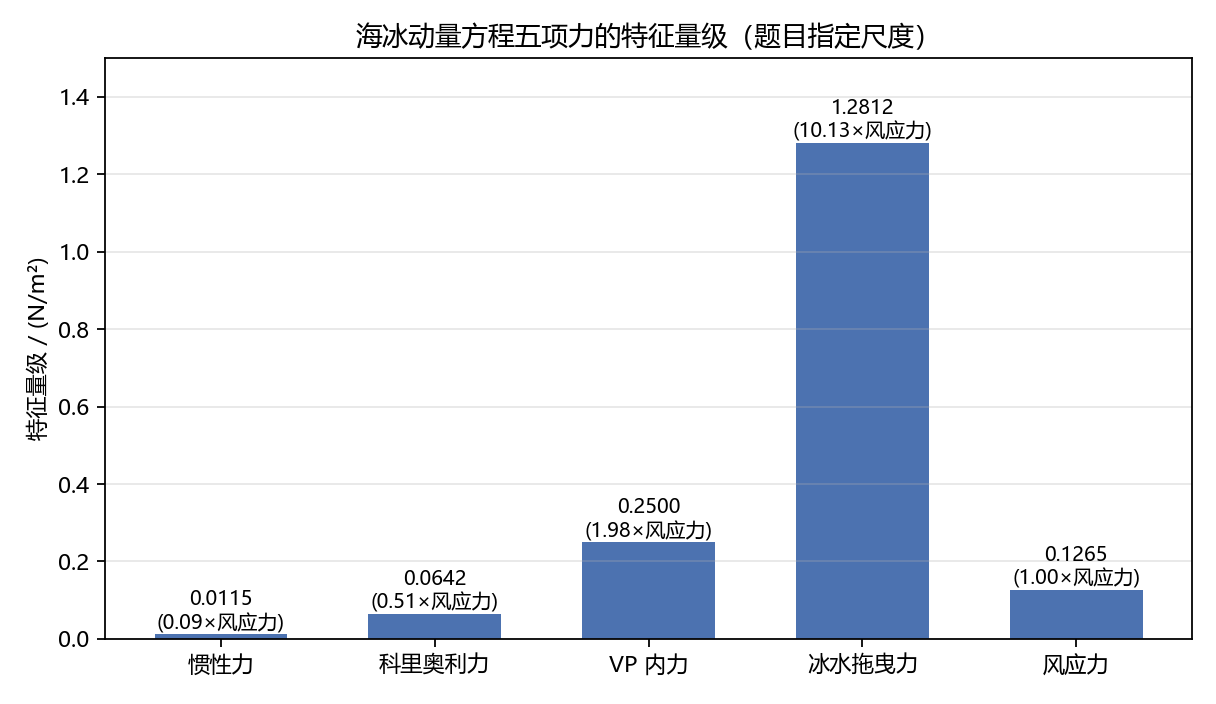
\includegraphics[width=0.72\textwidth]{figures/problem1_force_magnitudes.png}
\caption{海冰动量方程五项力的特征量级（题目指定尺度；惯性最小，海冰科里奥利与风应力仍属同量级）}
\label{fig:p1_force}
\end{figure}

两项待删力合计相对三项保留力合计仅为
\begin{equation}
\eta_{IC}=\frac{F_I+F_C}{F_\sigma+F_D+F_W}=4.5636\%.
\label{eq:eta_ic}
\end{equation}
式 \eqref{eq:eta_ic} 中的各个 $F$ 都是非负特征模长，因此 $\eta_{IC}$ 表示两类待删项的名义模长合计占三类保留项名义模长合计的比例。它只回答“在所取代表尺度下待删项相对多大”，不包含力的方向、空间分布和相消信息，更不是力平衡残差或场变量误差。M1 的实际结构代价仍需由共享初边值、空间离散和收敛标准的模型对照确定。

\subsection{模型选择：瞬时三力平衡 M1}

在候选方案层面，本文逐一考察三种简化：仅删惯性（保留海冰科里奥利）、仅删海冰科里奥利（保留惯性）、同时删两项。删除惯性后，无论是否保留海冰科里奥利，海冰动量方程都不再含时间导数，均属于准静态代数平衡；因此单项量级分析最直接支持的是仅删惯性的 $M_I$。题面后续明确要求使用双删项三力平衡形式，故本文把 $\eta_{IC}=4.5636\%$ 作为采用 M1 的启发式联合尺度指标，而不把它解释为解误差证明。题设 M1 为
\begin{equation}
0=\nabla\cdot(h_i\vect\sigma)+\vect\tau_{wi}+\vect\tau_a,
\label{eq:m1}
\end{equation}
并保留海水动量方程中的科里奥利力。该模型的合理性与代价应分开表述：一方面，代数平衡消除了海冰惯性时间推进，适合用 Picard 线性化结合稀疏线性求解器求取每个物理步的平衡状态；另一方面，VP 黏度、非线性拖曳和冰--水外层耦合仍需多次迭代，不能简化为“每步只解一次代数系统”。冰厚守恒与海水方程继续按真实时间推进，使海冰速度作为瞬时诊断量参与慢变量演化。M1 的采用依据是题设形式、计算可实现性和联合尺度指标的共同作用，其精度必须由 M0/$M_I$/$M_C$ 对照限定。

同时必须说明 M1 的代价：海冰科里奥利力本身并非可忽略的小量（为风应力的 $50.7\%$），删除它会移除海冰的直接科里奥利响应，仅保留海水经拖曳传递的间接影响。这在强剪切、冰缘与厚冰快速强迫场景可能造成方向与输运偏差，且对照误差已经超过 $5\%$ 参考线。因此后续问题按题意复用 M1，但不宣称其处于已验证的高精度适用域。

\subsubsection{M1 的分量形式与 VP 闭合}

将式 \eqref{eq:m1} 写成两个方向的平衡关系，有
\begin{align}
0={}&\frac{\partial(h_i\sigma_{xx})}{\partial x}
+\frac{\partial(h_i\sigma_{xy})}{\partial y}
+\rho_wC_dU_r(u-U)+\tau_{a,x},\\
0={}&\frac{\partial(h_i\sigma_{xy})}{\partial x}
+\frac{\partial(h_i\sigma_{yy})}{\partial y}
+\rho_wC_dU_r(v-V)+\tau_{a,y},
\end{align}
其中 $U_r=|\vect u-\vect U|$ 是冰水相对速度的模长，$u-U$ 与 $v-V$ 分别是相对速度在 $x,y$ 方向的分量；$\tau_{a,x},\tau_{a,y}$ 是风应力的两个水平分量。$\sigma_{xx},\sigma_{yy}$ 表示两个坐标方向上的正应力，$\sigma_{xy}=\sigma_{yx}$ 表示剪应力。VP 本构采用椭圆屈服曲线，冰强度为
\begin{equation}
P=P^*h_i\exp[-20(1-A)],
\qquad
A=\operatorname{clip}\left(\frac{h_i}{h_{i0}},0,1\right).
\end{equation}
令应变率不变量的正则化形式为
\begin{equation}
\Delta_\varepsilon=\sqrt{\Delta^2+\Delta_{\min}^2},
\qquad
\zeta=\min\left(\frac{P}{2\Delta_\varepsilon},\zeta_{\max}\right),
\qquad
\eta=\frac{\zeta}{e^2},
\end{equation}
则应力可写成应变率的非线性函数。这里，$\Delta$ 汇总拉伸、压缩和剪切应变率，$\Delta_\varepsilon$ 是其正则化值；$\zeta$ 与 $\eta$ 分别为体黏度和剪切黏度，椭圆率 $e$ 控制两者比例；$\Delta_{\min}$ 防止分母在近刚性区趋于零，$\zeta_{\max}$ 限制黏度上界。后二者属于数值正则化参数，只用于使非线性方程可稳定求解，不增加新的外力，也不改变 M1 保留的三类物理作用。

\subsection{模型对比实验：双删项结构差异与归因}

为检验简化代价并解释差异来源，在 $40\times20$、$\Delta t=300\ \mathrm s$、6 h 的同一离散框架下（共享全部方程、参数、残差与求解器配置，仅切换惯性权重与海冰科里奥利权重），运行完整模型 M0、仅删惯性的 $M_I$、仅删海冰科里奥利的 $M_C$ 与双删项 M1 四个模型，相对 M0 的结构差异见表 \ref{tab:p1_attr} 与图 \ref{fig:p1_attr}。差异指标定义为 $\|\cdot\|_2/\|\cdot\|_2$ 型相对误差，分别考察终时速度场、全过程时空速度场、终时冰厚场与全过程时空冰厚场。

\begin{table}[H]
\centering
\caption{四模型相对 M0 的结构差异（40×20、6 h）}
\renewcommand{\arraystretch}{1.4}
\begin{tabular*}{\textwidth}{
    @{\extracolsep{\fill}}
    l
    c
    c
    c
    c
    @{}
}
\toprule[1pt]
模型 & 终时速度 & 时空速度 & 终时冰厚 & 时空冰厚\\
\midrule
$M_I$（仅删惯性） & $4.669\%$ & $9.543\%$ & $2.482\%$ & $2.507\%$\\
$M_C$（仅删科里奥利） & $10.103\%$ & $8.274\%$ & $10.573\%$ & $6.717\%$\\
M1（双删） & $11.190\%$ & $12.777\%$ & $11.600\%$ & $7.855\%$\\
\bottomrule[1pt]
\end{tabular*}
\label{tab:p1_attr}
\end{table}

\begin{figure}[H]
\centering
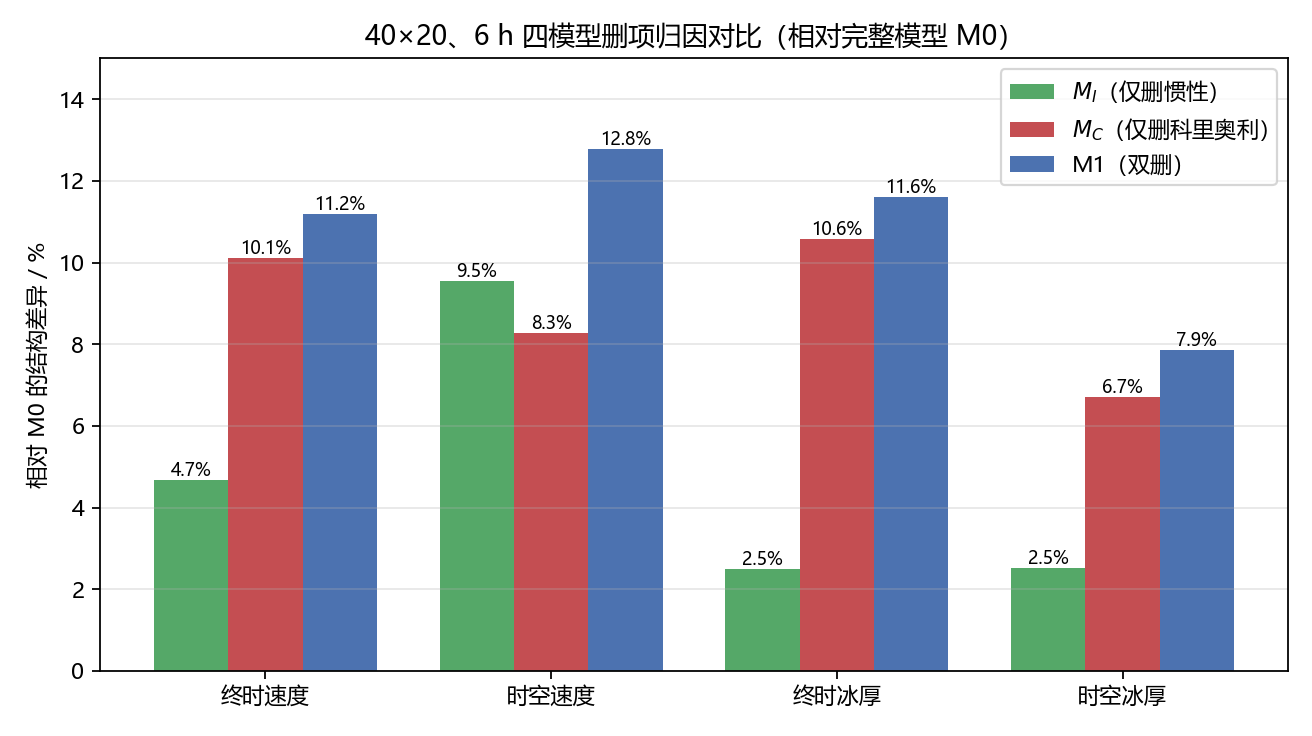
\includegraphics[width=0.86\textwidth]{figures/problem1_attribution.png}
\caption{四模型相对 M0 的结构差异对比（40×20、6 h；双删项 M1 的差异接近但略小于单删项之和，交互占比中等）}
\label{fig:p1_attr}
\end{figure}

对比结果揭示了三层信息。第一，删除海冰科里奥利后，终时冰厚差异达到 $10.573\%$，说明速度方向的改变会经守恒输运逐步累积；删除惯性后，时空速度差异为 $9.543\%$，表明启动和调整过程仍会影响全过程速度。第二，双删项 M1 的四项差异均小于两个单删项差异之和，速度终时的相对交互占比 $q=0.3105$，说明两类作用之间存在非线性交互，不能把两个百分数直接相加。第三，M1 在该诊断场景中的结构差异为 $7.9\%$--$12.8\%$，超过预先设置的 $5\%$ 比较线。该结果不改变题目指定 M1 的模型身份，但说明其并非在所有海况下都与完整动力模型接近。

\subsection{实际离散力预算与数值归因}

特征量级以代表性尺度估算，无法反映真实离散场中的空间非均匀性。为此，本文在最严格的 D 组（$40\times20$、$\Delta t=150\ \mathrm s$，残差阈值收紧 10 倍）中，对 M0 每个已接受物理状态计算实际力预算。按本文符号约定，完整方程右端的海冰科里奥利力为 $\vect F_C=-\rho_i h_if\vect k\times\vect U$，因此 M1 相对 M0 缺失的向量合量是 $\vect F_I-\vect F_C$；无方向的尺度筛查则使用 $|\vect F_I|+|\vect F_C|$。两者不能混用。

\begin{table}[H]
\centering
\caption{严格 D/M0 离散力预算统计}
\renewcommand{\arraystretch}{1.35}
\begin{tabular*}{\textwidth}{@{\extracolsep{\fill}}lccc@{}}
\toprule[1pt]
指标 & 中位数 & 95\% 分位数 & 最大值\\
\midrule
$|\vect F_I-\vect F_C|$/$(\mathrm{N/m^2})$ & $0.008882$ & $0.031273$ & $0.125039$\\
$|\vect F_I|+|\vect F_C|$/$(\mathrm{N/m^2})$ & $0.009435$ & $0.035531$ & $0.127632$\\
$|\vect F_\sigma|+|\vect F_D|+|\vect F_W|$/$(\mathrm{N/m^2})$ & $0.252608$ & $0.262172$ & $0.351767$\\
$r_{IC}=|\vect F_I-\vect F_C|/(|\vect F_\sigma|+|\vect F_D|+|\vect F_W|)$ & $3.535\%$ & $12.210\%$ & $94.021\%$\\
\bottomrule[1pt]
\end{tabular*}
\label{tab:p1_force_budget}
\end{table}

中位数 $3.535\%$ 与名义指标 $4.5636\%$ 同量级，说明特征尺度判断能够描述主体区域；但 95\% 分位数已升至 $12.210\%$，最大值更受局部近抵消和小分母放大影响。这一长尾分布解释了为什么“平均量级较小”不能推出“全场结构差异小于 $5\%$”。

进一步设置 A--D 四组对照：A 为正式时间步与正式残差，B 仅收紧残差，C 仅将时间步减半，D 同时收紧残差并减半时间步。结果见表 \ref{tab:p1_abcd}。

\begin{table}[H]
\centering
\caption{残差与时间步对 M1--M0 结构差异的影响（40×20、6 h）}
\renewcommand{\arraystretch}{1.35}
\begin{tabular*}{\textwidth}{@{\extracolsep{\fill}}lcccc@{}}
\toprule[1pt]
组别 & 终时速度 & 时空速度 & 终时冰厚 & 时空冰厚\\
\midrule
A：$\Delta t=300$ s，正式残差 & $11.190\%$ & $12.777\%$ & $11.600\%$ & $7.855\%$\\
B：$\Delta t=300$ s，严格残差 & $11.190\%$ & $12.777\%$ & $11.600\%$ & $7.855\%$\\
C：$\Delta t=150$ s，正式残差 & $11.065\%$ & $13.444\%$ & $11.544\%$ & $7.778\%$\\
D：$\Delta t=150$ s，严格残差 & $11.066\%$ & $13.444\%$ & $11.544\%$ & $7.778\%$\\
\bottomrule[1pt]
\end{tabular*}
\label{tab:p1_abcd}
\end{table}

收紧残差后 A 与 B 几乎重合；时间步减半后，M0 与 M1 各自相对 D 组的变化均不超过约 $1.1\%$，而两模型之间的差异仍明显高于 $5\%$。因此，这一差异主要来自方程结构，而不是当前求解容差或时间离散。后续求解器优化只改变收敛路径和计算成本，不应被解释为对物理删项误差的修正。

\begin{figure}[H]
\centering
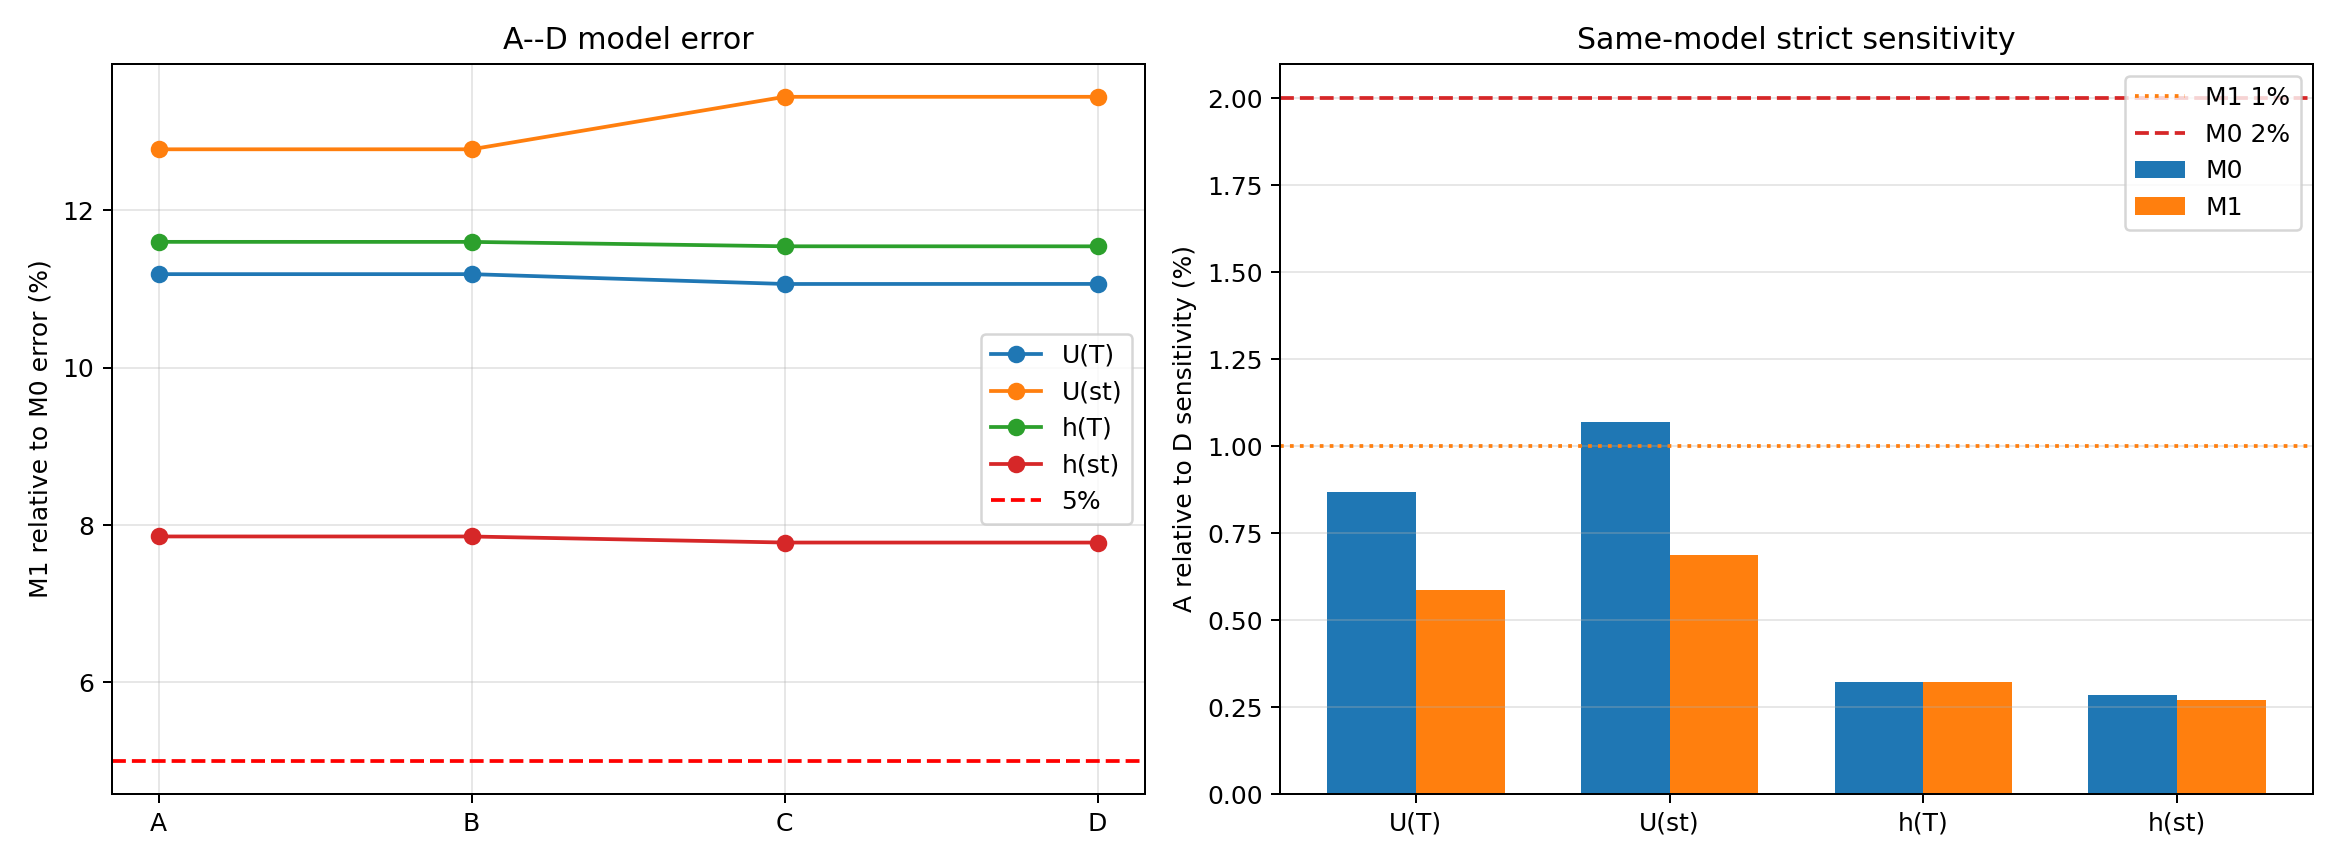
\includegraphics[width=0.84\textwidth]{figures/problem2_diagnostic_error_sensitivity.png}
\caption{A--D 组结构差异对残差与时间步的敏感性（虚线为 5\% 比较线）}
\label{fig:p1_abcd}
\end{figure}

\subsection{碎冰区、厚冰区与适用边界}

在碎冰区（$h_i\to0$），各项力的尺度随冰厚变化：惯性力与海冰科里奥利力均为 $O(h_i)$，而厚度加权 VP 内力 $\sim h_i P/L$ 中 $P=P^*h_i\exp[-20(1-A)]$，当 $A\to0$ 时指数项 $\exp(-20)$ 使内力按 $O(h_i^2)$ 衰减，衰减更快。因此碎冰区中“惯性/科里奥利相对 VP 内力”的占比反而上升，简化前提（待删力远小于保留力）被削弱；加之稀疏碎冰偏离连续介质假设，$h_i<h_{\min}$ 时本文直接启用无冰掩膜，避免在碎冰区强行使用 M1。

在厚冰区（$A=1$），$P=P^*h_i$，冻结应变尺度和局部变化尺度时，厚度加权 VP 内力量级近似随 $h_i^2$ 增长，而惯性与科里奥利力量级随 $h_i$ 线性增长。这说明厚冰区必须保留 VP 内力，但不能据此断言双删项一定更准确：厚冰具有更长的动力调整时间，固壁和挤压带附近还容易形成强应力梯度，快速强迫下完整模型与瞬时平衡模型仍可能产生明显差异。

综合量级分析与对照实验，M1 更适合用于\textbf{外力变化较缓、连续冰盖假设尚可、保留力未发生强抵消}的诊断场景。快速强迫（如风场突变）、初始失衡（速度场未达到准平衡）、低冰水相对速度（拖曳趋零导致三力平衡退化为二力平衡）、外力近抵消（平衡方程病态）、边界强剪切与冰缘裂隙均可能放大 M1 与 M0 的结构差异，属于简化模型需要谨慎使用的边界。后续各问按题意继续采用 M1 作为正演内核，并将上述机制视为共同的适用性限制，而不声称所有后续场景已经落入其高精度范围。

\section{问题二：海冰--海水耦合模型的数值求解}

\subsection{问题分析}

问题二需要把 M1 的瞬时力平衡嵌入随时间演化的冰--水系统。其难点并不只是方程规模大，而是三个时间尺度同时存在：海水表面重力波传播最快，海冰速度通过非线性 VP 平衡迅速调整，冰厚则在平流作用下缓慢变化。表面重力波相速约为 $\sqrt{gh_w}=17.1\ \mathrm{m/s}$，在题定 $100\ \mathrm m$ 网格与 $300\ \mathrm s$ 时间步下，显式重力波 CFL 数约为 51；与此同时，零应变率附近的 VP 黏度趋于无穷，冰水拖曳又依赖未知相对速度。因此，数值方案必须同时处理快波稳定性、非线性流变和界面耦合，并在 288 个物理步内保持质量守恒和可接受的计算成本。

\subsection{模型与离散}

正式求解模型为式 \eqref{eq:m1} 与冰厚守恒方程、海水浅水方程：
\begin{align}
&\frac{\partial h_i}{\partial t}+\nabla\cdot(h_i\vect U)=0,\\
&\frac{\partial\xi}{\partial t}+\nabla\cdot[(h_w+\xi)\vect u]=0,\\
&\frac{\partial\vect u}{\partial t}+(\vect u\cdot\nabla)\vect u
=-g\nabla\xi-f(\vect k\times\vect u)-\frac{\vect\tau_{wi}}{\rho_wh_w}.
\end{align}
其中，$h_i$ 是需要随速度场输运的海冰厚度；$\xi$ 表示相对于静止水面的自由面位移，$h_w+\xi$ 是局地总水深；$g\nabla\xi$ 为海面倾斜产生的压力梯度；海水科里奥利项 $f(\vect k\times\vect u)$ 在 M1 中仍然保留；$-\vect\tau_{wi}/(\rho_wh_w)$ 是海冰对海水的反作用加速度。冰厚方程没有源汇项，意味着闭域内冰的总体积只会在网格间重新分配而不会凭空增加或减少。
空间采用 C 型交错网格：冰厚、海面高度定义在单元中心，速度定义在法向面，这是海洋模式中常用的压力--速度排布\cite{arakawa1977}，可避免棋盘式压力振荡。VP 应力的离散遵循“中心--角点”闭合链：先在中心计算 $\dot\epsilon_{xx},\dot\epsilon_{yy}$，将四个角点的 $\dot\epsilon_{xy}^2$ 平均到中心后计算不变量 $\Delta$、黏度 $\zeta,\eta$ 与正应力 $h_i\sigma_{xx},h_i\sigma_{yy}$，再将中心 $\eta$ 平均回角点计算剪应力 $h_{i,c}\sigma_{xy,c}$；散度计算与矩阵装配使用同一算子，保证“离散的 $\nabla\cdot(h_i\vect\sigma)$”与线性系统严格一致。VP 奇异通过正则化 $\Delta_\varepsilon=\sqrt{\Delta^2+\Delta_{\min}^2}$ 与黏度上限 $\zeta_{\max}$ 处理。冰厚输运采用守恒型迎风格式并受 CFL 限制（$\Delta t$ 内冰速最大位移不超过 0.8 倍网格距）。边界条件按题面：海冰固壁无滑移（法向速度为零、切向奇延拓）、海水自由滑移（法向速度为零、切向偶延拓）、冰厚零法向通量。

\subsubsection{C 网格变量配置}

交错排布使压力梯度、速度散度和界面通量天然位于相邻控制体上。各变量的位置与作用见表 \ref{tab:cgrid}。

\begin{table}[H]
\centering
\caption{C 型网格上的主要变量配置}
\renewcommand{\arraystretch}{1.35}
\begin{tabular*}{\textwidth}{@{\extracolsep{\fill}}lll@{}}
\toprule[1pt]
位置 & 变量 & 主要离散作用\\
\midrule
单元中心 $(i,j)$ & $h_i,\xi,A,P,\sigma_{xx},\sigma_{yy}$ & 质量守恒、海面连续方程和法向应力\\
$x$ 法向面 $(i+\tfrac12,j)$ & $U,u$ & $x$ 向动量、质量通量与压力梯度\\
$y$ 法向面 $(i,j+\tfrac12)$ & $V,v$ & $y$ 向动量、质量通量与压力梯度\\
单元角点 $(i+\tfrac12,j+\tfrac12)$ & $\dot\epsilon_{xy},\sigma_{xy}$ & 剪切应变与剪切应力通量\\
\bottomrule[1pt]
\end{tabular*}
\label{tab:cgrid}
\end{table}

其中速度模长并不直接定义在 C 网格面上。本文将 $U,V$ 分别插值到单元中心后计算 $|\vect U|$，并把该值称为“单元中心插值冰速”；面速度分量的最大值仅作为数值诊断，避免两种统计口径混淆。

\subsubsection{单步冰水耦合流程}

每个物理时间步按以下顺序推进：
\begin{enumerate}
\item 由前两个已接受状态预测新的海冰、海水初值；若掩膜变化或预测异常，则回退到上一时刻状态；
\item 固定海水速度和冰厚，以 Picard 法更新 VP 黏度与拖曳系数，并用 GMRES/ILU 求解线性化海冰平衡；
\item 由收敛海冰速度计算唯一的界面拖曳对象，在海冰和海水方程中以等大反向形式使用；
\item 对海水平流项显式推进，对重力波和海面高度采用 IMEX--Helmholtz 隐式更新；
\item 在外层固定点上比较冰速、海水速度和界面拖曳，利用受保护 Anderson 组合加速，达到耦合残差后接受该状态；
\item 用接受的海冰面通量守恒更新冰厚，并检查非负性、CFL、冰量、海面均值和边界通量。
\end{enumerate}
这种分块流程避免一次装配包含所有变量的超大雅可比矩阵，同时确保拖曳闭合和冰厚守恒在离散层面可核验。

\subsection{算法选择与理由}

海冰子系统的非线性来自 VP 黏度与拖曳系数对速度的依赖。正式 24 h 结果采用\textbf{Picard 线性化 + GMRES/ILU}：Picard 避免显式推导 Newton 黏度雅可比，GMRES 则可覆盖统一 M0/M1 框架中可能出现的非对称线性系统\cite{zhang1997,saad2003}。需要区分“通用框架”与“本次 M1 实例”：经矩阵检查，本次冻结的 M1 线性矩阵为对称矩阵，因而“矩阵必然非对称、迭代法必然优于直接法”并不成立；$40\times20$、6 h 对照中稀疏直接 LU 反而最快。EVP/mEVP 伪时间迭代\cite{hunke1997}便于并行，但需另行标定子步数与阻尼，当前未作为正式生产路线。海水方程采用 IMEX（显式平流、隐式正压）与 Helmholtz 求解\cite{ascher1997}，把表面重力波从显式 CFL 中移出；冰水拖曳应力在冰水两侧共享同一离散对象，保证离散动量闭合。

\begin{table}[H]
\centering
\caption{问题二主要数值方法的比较}
\renewcommand{\arraystretch}{1.35}
\begin{tabular*}{\textwidth}{@{\extracolsep{\fill}}p{2.4cm}p{2.9cm}p{2.9cm}p{3.1cm}@{}}
\toprule[1pt]
环节 & 备选方法 & 主要问题 & 采用方案\\
\midrule
VP 非线性 & Newton、Picard、EVP/mEVP & Newton 雅可比复杂；EVP 需标定伪时间子步 & Picard 稳健线性化，保留 EVP/mEVP 为并行扩展\\
线性系统 & 直接 LU、CG、BiCGSTAB、GMRES & 直接法高网格填充大；CG 要求正定；BiCGSTAB 长时稳健性待检验 & GMRES/ILU 作为统一主线，小网格 LU 作实现对照\\
浅水快模态 & 全显式、全隐式、IMEX & 全显式 CFL 失稳；全隐式单步代价高 & IMEX--Helmholtz 隐式处理重力波\\
冰厚输运 & 中心差分、迎风、TVD/WENO & 中心格式易振荡；高阶格式实现与边界复杂 & 守恒一阶迎风，优先保证非负与质量守恒\\
耦合迭代 & 松弛、Aitken、Anderson & 纯松弛收敛慢；加速可能病态 & Aitken 基线与受保护 Anderson\\
\bottomrule[1pt]
\end{tabular*}
\label{tab:p2_method_compare}
\end{table}

\subsection{求解器优化与对比实验}

为降低正式计算成本，在保持 M1 方程、离散、参数、容限与输出不变的前提下，依次引入三种受保护优化。它们在残差上升、数值病态、掩膜变化或矩阵漂移时回退；是否保持同一离散解不靠设计口号保证，而由优化前后固定点误差对照验收：

\begin{enumerate}
\item \textbf{时间预测初值：}由最近两个已接受状态线性外推下一步初值。准静态 M1 的每一步求解本质上是“从旧平衡到新平衡”的连续变形，线性外推给出的初值比旧状态更接近新固定点，可显著减少外层耦合迭代；掩膜或数值保护条件触发时回退到旧状态。
\item \textbf{受保护外层 Anderson 加速：}对冰--水外层固定点迭代做块归一化 Anderson 组合（深度 3、阻尼 0.8）\cite{walker2011}。Anderson 用最近几次残差的线性组合构造加速方向，对强非线性耦合的收敛加速显著；其风险是组合系数病态，因此设置残差上升、条件数超限、非有限或掩膜变化的触发条件，触发即清空历史并回退 Aitken 松弛。
\item \textbf{受保护 ILU 复用：}同一物理步、同一耦合轮次内相邻 Picard 迭代复用 ILU 预条件器（最多 2 次）。Picard 迭代中矩阵随速度场缓慢变化，ILU 频繁重建是主要开销；在矩阵漂移、稀疏模式变化或 GMRES 退化时立即重建，保证预条件质量不下降。
\end{enumerate}

优化效果通过 $40\times20$、24 h 的三组交错重复计时对照（表 \ref{tab:p2_opt}）。

\begin{table}[H]
\centering
\caption{求解器优化前后对照（40×20、24 h，各 3 次）}
\renewcommand{\arraystretch}{1.4}
\begin{tabular*}{\textwidth}{
    @{\extracolsep{\fill}}
    l
    c
    c
    c
    c
    @{}
}
\toprule[1pt]
指标 & 未优化 & 时间预测+Anderson & +ILU 复用 & 最终变化\\
\midrule
墙钟中位数 / s & $504.787$ & $420.081$ & $395.899$ & $-21.6\%$\\
外层耦合总迭代 & $6578$ & $3547$ & $3547$ & $-46.1\%$\\
Picard 总迭代 & $17466$ & $15221$ & $15221$ & $-12.9\%$\\
GMRES 总迭代 & $54866$ & $50433$ & $50433$ & $-8.1\%$\\
重试步+额外尝试 & $2+2$ & $3+3$ & $3+3$ & --\\
\bottomrule[1pt]
\end{tabular*}
\label{tab:p2_opt}
\end{table}

表 \ref{tab:p2_opt} 显示：外层耦合迭代下降 $46.1\%$，是 24 h 墙钟下降的主要来源；Picard 与 GMRES 总迭代分别下降 $12.9\%$ 与 $8.1\%$。优化版相对基线的四类场差异最大为 $0.0228\%$，低于预设 $0.1\%$ 数值等价门槛，支持两者在规定容差内收敛到等价的离散固定点。表中的“重试步”是首次尝试未满足冻结残差后，由保护策略重新求解并最终接受的物理步；它不改变方程或验收阈值，但应计入实际墙钟与稳健性评价。

为判断线性求解与装配层的进一步改进是否值得采用，另在同一 $40\times20$ 网格上做 6 h 实现级对照（表 \ref{tab:p2_impl}）。这里的 P4 是旧版参考，后三行依次累计零项剪枝、安全稀疏模式/预条件信息复用和稀疏直接 LU；该表只证明小网格短时段的实现等价与速度收益，不替代 24 h 正式验证，也不外推至 $200\times100$。

\begin{table}[H]
\centering
\caption{实现级求解器对照（40×20、6 h）}
\renewcommand{\arraystretch}{1.35}
\begin{tabular*}{\textwidth}{@{\extracolsep{\fill}}lccc@{}}
\toprule[1pt]
实现版本 & 墙钟/s & 相对 P4 加速 & 最大固定点差异\\
\midrule
P4 旧参考 & $91.829$ & $1.000$ & --\\
零项剪枝 & $39.421$ & $2.329$ & $2.78\times10^{-13}$\\
安全复用 & $37.501$ & $2.449$ & $6.94\times10^{-8}$\\
稀疏直接 LU & $33.605$ & $2.733$ & $2.06\times10^{-8}$\\
\bottomrule[1pt]
\end{tabular*}
\label{tab:p2_impl}
\end{table}

作为补充，对第一个 $200\times100$ 线性系统（$40300\times40300$、非零元约 $3.6\times10^5$）比较 GMRES 与 BiCGSTAB：两者均达到 $10^{-8}$ 相对残差，单步墙钟分别为 $4.35\ \mathrm s$ 与 $2.15\ \mathrm s$。这说明 BiCGSTAB 在该单系统上更快，但单步测试不能代表 288 步长时程稳健性；正式 24 h 数据仍来自 GMRES/ILU，直接 LU 仅作为后续实现改进候选。

\subsection{两网格结果一致性与可完成网格结果}

题面规定 $200\times100$ 网格；受竞赛限时与单机算力约束，该网格 24 h 全时段未完成。本文在可完成的 $100\times50$ 替代网格（$\Delta x=\Delta y=200\ \mathrm m$）上给出结果，并与 $40\times20$ 网格做选定统计量的一致性检查（表 \ref{tab:p2_grid}）。区域平均冰厚恒为 $0.5\ \mathrm m$ 主要来自闭域零通量下的质量守恒，不能用作网格收敛证据；两套网格也不足以估计收敛阶。因此本节不宣称完成题定网格或严格网格收敛。

\begin{table}[H]
\centering
\caption{两网格 M1 24 h 结果对比}
\small
\setlength{\tabcolsep}{3pt}
\renewcommand{\arraystretch}{1.4}
\begin{tabular*}{\textwidth}{
    @{\extracolsep{\fill}}
    l
    c
    c
    c
    c
    c
    c
    @{}
}
\toprule[1pt]
网格 & 完成步 & 平均冰厚/m & 终时中心速度/(m/s) & 中心冰厚/m & 冰体积误差 & 墙钟/s\\
\midrule
$40\times20$ & $288/288$ & $0.500000$ & $0.208264$ & $0.844796$ & $1.5\times10^{-16}$ & $395.899$\\
$100\times50$ & $288/288$ & $0.500000$ & $0.208846$ & $0.849975$ & $1.5\times10^{-16}$ & $15395.6$\\
\bottomrule[1pt]
\end{tabular*}
\label{tab:p2_grid}
\end{table}

两网格区域平均冰厚严格一致（$0.500000\ \mathrm m$，闭域零通量下解析上应守恒），终时单元中心重构最大冰速之比为 $1.0028$，中心点冰厚差异约 $0.6\%$。这些结果只表明所比较的三个标量呈现一致性迹象；它们既不包含全场误差范数，也不足以证明网格收敛或估计空间收敛阶。$100\times50$ 网格的统计量与场图如下。

\begin{table}[H]
\centering
\caption{100×50 可完成替代网格 24 h 统计量（6 位小数）}
\renewcommand{\arraystretch}{1.4}
\begin{tabular*}{\textwidth}{
    @{\extracolsep{\fill}}
    l
    c
    @{}
}
\toprule[1pt]
指标 & 数值\\
\midrule
24 h 区域平均冰厚 / m & $0.500000$\\
24 h 单元中心重构最大冰速 / (m/s) & $0.208846$\\
全时段运行诊断最大冰速 / (m/s) & $0.218550$\\
最大冰速中心坐标 / m & $(11500,1300)$\\
24 h 中心点 (10000,5000) 冰厚 / m & $0.849975$\\
冰体积相对误差 & $1.5\times10^{-16}$\\
\bottomrule[1pt]
\end{tabular*}
\label{tab:p2_formal}
\end{table}

替代网格结果为：区域平均冰厚 $0.500000\ \mathrm m$、终时单元中心重构最大冰速 $0.208846\ \mathrm{m/s}$（均保留 6 位小数），冰体积相对误差 $1.5\times10^{-16}$。288 个物理步最终均被接受，其中 113 个物理步经过保护性重试，累计增加 120 次求解尝试。重试没有修改 M1 方程、残差阈值或守恒判据，但表明更细网格显著增加了非线性耦合的刚性与计算负担。为避免只用最终场判断数值质量，表 \ref{tab:p2_quality} 汇总全过程的硬检查。

\begin{table}[H]
\centering
\caption{100×50、24 h 正演的数值质量指标}
\renewcommand{\arraystretch}{1.35}
\begin{tabular*}{\textwidth}{@{\extracolsep{\fill}}lccc@{}}
\toprule[1pt]
指标 & 计算值 & 控制阈值 & 判定\\
\midrule
最大海冰动量残差 & $9.977\times10^{-4}$ & $10^{-3}$ & 通过\\
最大 GMRES 相对残差 & $9.988\times10^{-9}$ & $10^{-8}$ & 通过\\
最大冰水耦合残差 & $9.998\times10^{-6}$ & $10^{-5}$ & 通过\\
最大海水方程残差 & $9.971\times10^{-9}$ & $10^{-8}$ & 通过\\
最大 Helmholtz 残差 & $1.476\times10^{-13}$ & $10^{-8}$ & 通过\\
最大冰厚 CFL 数 & $0.468$ & $0.8$ & 通过\\
冰体积相对误差 & $1.49\times10^{-16}$ & $10^{-6}$ & 通过\\
最小冰厚 / m & $9.61\times10^{-13}$ & $\ge0$ & 通过\\
\bottomrule[1pt]
\end{tabular*}
\label{tab:p2_quality}
\end{table}

这些指标说明该次离散运行在既定方程和网格上满足冻结残差、非负性、CFL 与守恒要求，但 113 个重试步也显示其求解稳健性仍有改进空间。上述数值质量检查不能替代题定 $200\times100$ 网格输出，也不能消除问题一所揭示的 M1 结构差异。

\begin{figure}[H]
\centering
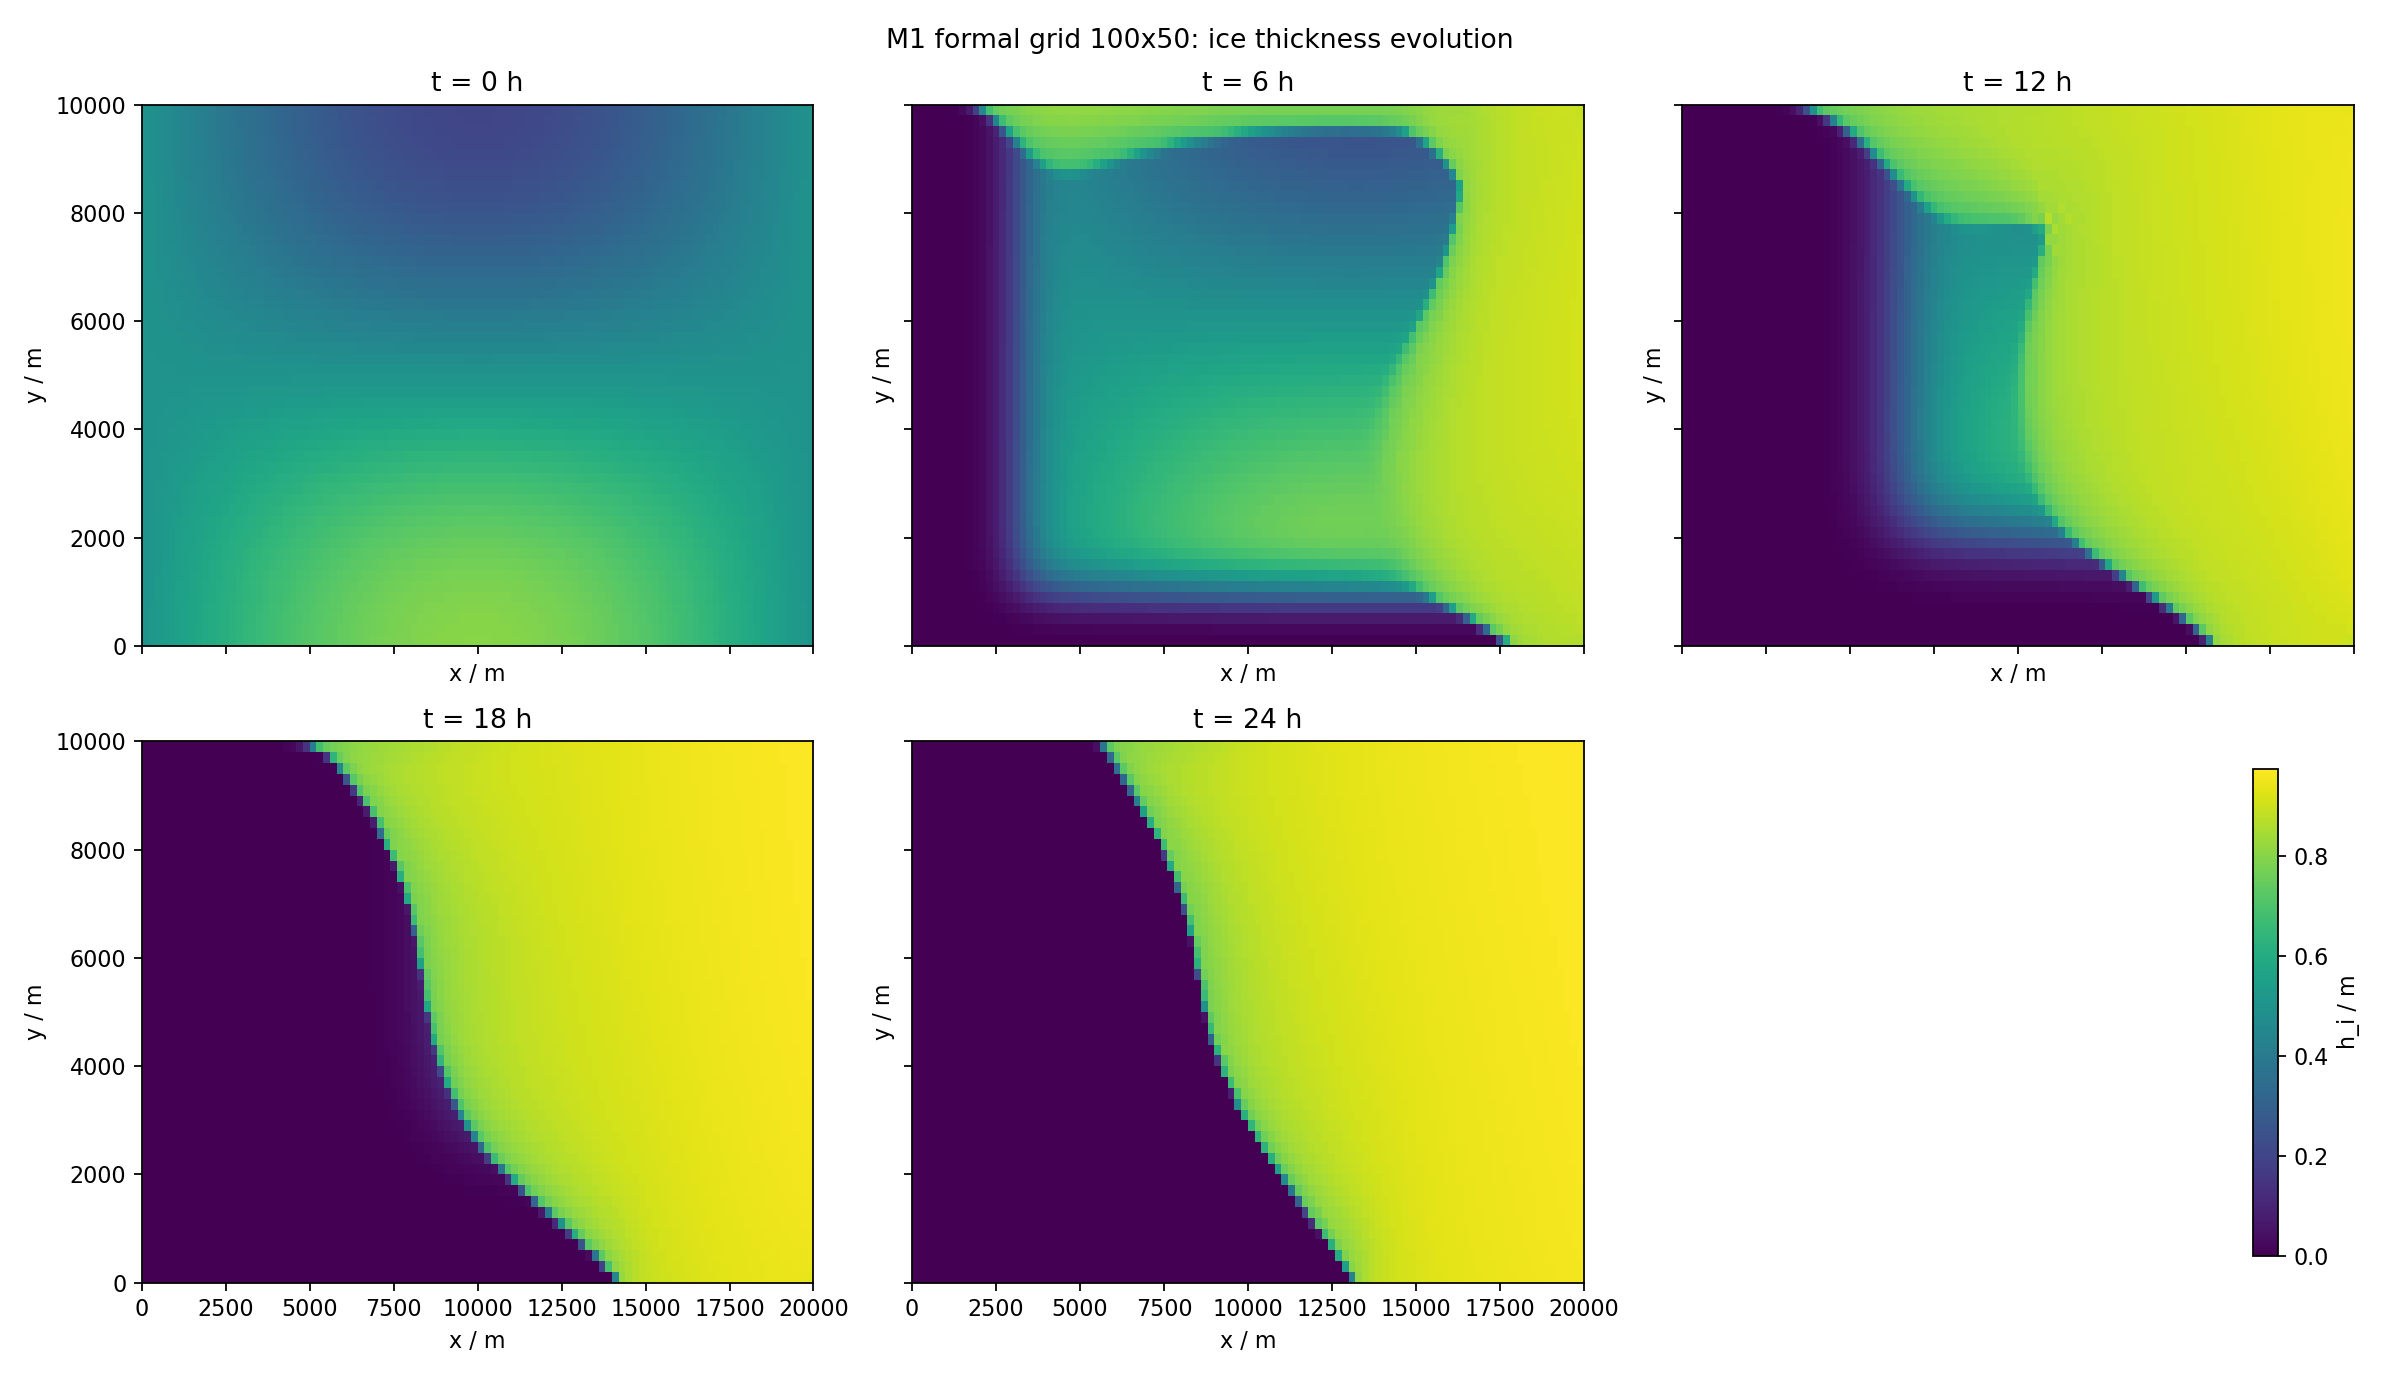
\includegraphics[width=0.93\textwidth]{figures/problem2_thickness_evolution.png}
\caption{100×50 M1 24 h 冰厚场演化}
\label{fig:p2_evo}
\end{figure}

\begin{figure}[H]
\centering
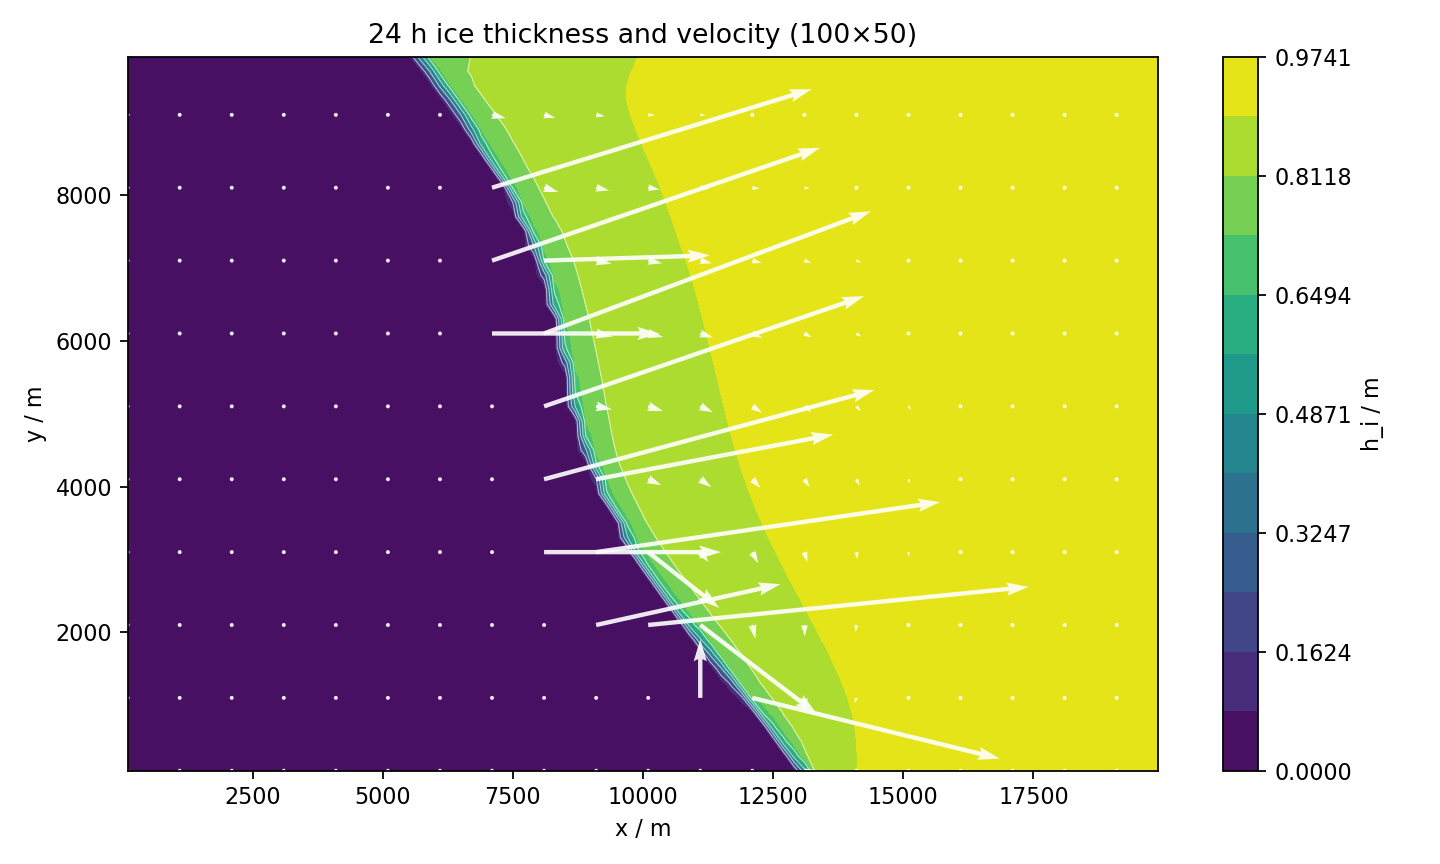
\includegraphics[width=0.88\textwidth]{figures/problem2_thickness_contour_velocity_24h.png}
\caption{100×50 M1 24 h 冰厚等值线与冰速矢量}
\label{fig:p2_vel}
\end{figure}

\begin{figure}[H]
\centering
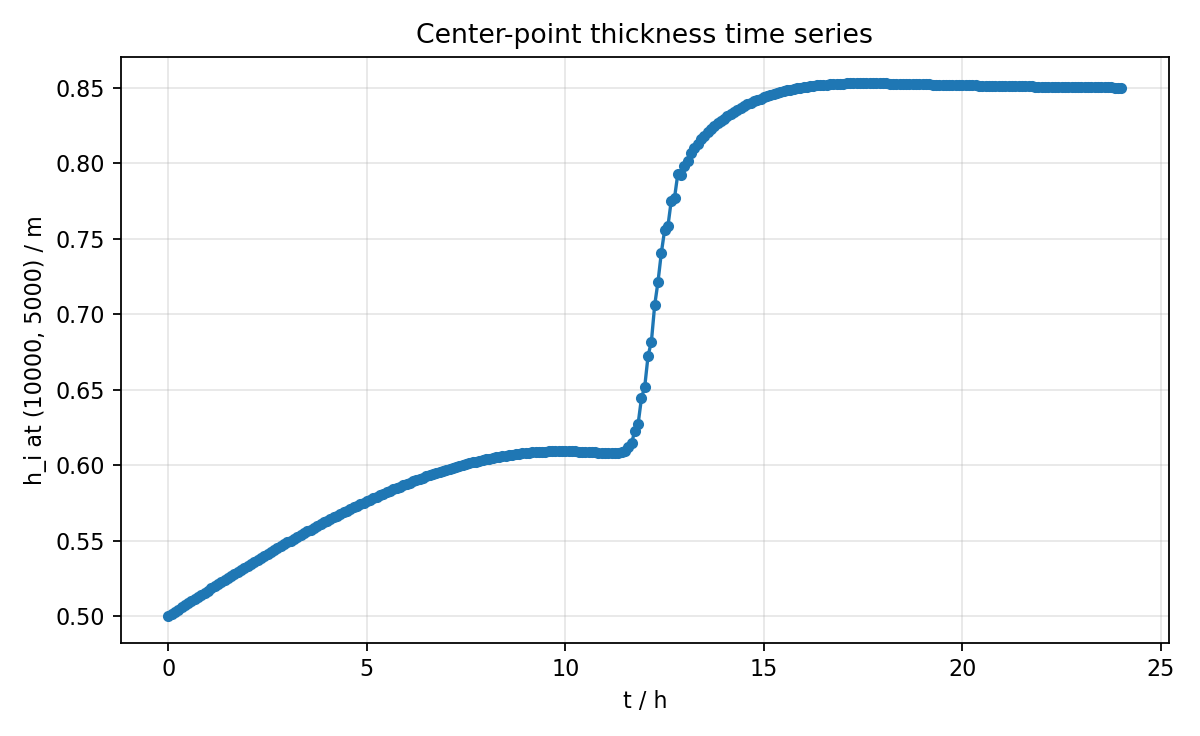
\includegraphics[width=0.72\textwidth]{figures/problem2_center_thickness_timeseries.png}
\caption{海域中心点 (10000,5000) 冰厚随时间变化}
\label{fig:p2_center}
\end{figure}

冰速场总体表现为薄冰及厚度梯度较大区域速度偏高、厚冰主体内部速度偏低。终时单元中心重构最大冰速为 $0.208846\ \mathrm{m/s}$，位置为 $(11500,1300)$，邻近冰厚梯度较明显区域。这种空间共现与风应力、冰水拖曳和 VP 内力共同平衡的机制相容，但尚未对该点逐项分解力预算，不能据此判定某一力为主因。

中心厚冰区速度相对较低，与冰强度随厚度增加、内部应力传递增强的总体机制一致。由于 M1 删除了海冰直接科里奥利项，冰速方向的偏转主要由保留海水科里奥利的浅水方程产生，再通过冰水拖曳间接传递。中心点冰厚由初值约 $0.8\ \mathrm m$ 增至 $0.849975\ \mathrm m$；结合中心点周围净通量，该位置在 24 h 内表现为局部辐合堆积。

\section{问题三：冰水拖曳系数与风应力缩放系数的参数反演}

\subsection{问题分析}

冰水拖曳系数 $C_d$ 控制海冰趋近海流的强度，风应力缩放系数 $\alpha$ 控制大气强迫幅值；二者均能改变冰速大小，因而可能沿相互补偿的方向形成狭长目标谷地。虽然本问只有两个未知参数、共有 12 个观测分量，但观测数量多于参数数量并不意味着参数一定可辨识：若不同参数组合产生相近冰速，或前向模型存在系统方向偏差，目标函数仍会平坦或在边界处取到最小值。本文采用全域采样、局部无导数搜索和种群进化三类方法交叉求解，并利用模型一致的孪生试验区分“优化器识别能力不足”和“真实观测与模型不一致”两种原因。

\subsection{观测误差模型与目标函数}

以订正后的 M1 内核为前向模型，利用 6 个位置 t=24 h 冰速观测反演 $C_d$ 与 $\alpha$。固壁观测点 (20000,7500) 处海冰无滑移速度为 0，观测值与其矛盾属观测误差，本文按观测误差模型将其方差放大 100 倍（$\sigma=0.10\ \mathrm{m/s}$），内部点取 $\sigma=0.01\ \mathrm{m/s}$，不修改观测值与边界条件。目标函数为加权最小二乘
\begin{equation}
J(C_d,\alpha)=\sum_{k=1}^{6}
\frac{(U_k^{\mathrm{obs}}-U_k^{\mathrm{mod}})^2+(V_k^{\mathrm{obs}}-V_k^{\mathrm{mod}})^2}{\sigma_k^2}.
\end{equation}
该目标函数是各站点残差平方的方差归一化加权和，$\sigma_k$ 越小权重越大。固壁点处理遵循“\textbf{误差建模而非数据修改}”原则：观测值 (0.04,0.08) 与无滑移预测 0 矛盾，是边界条件与真实观测机制的系统差异，直接拟合会迫使反演参数去补偿边界结构误差，反而污染内部点的参数识别；将方差放大 100 倍后，该点权重降至内部点的 1/100，反演以内部 5 点为主导，同时不隐瞒固壁点的残差信息。

式中 $U_k^{\mathrm{obs}},V_k^{\mathrm{obs}}$ 是第 $k$ 个站点的观测速度分量，$U_k^{\mathrm{mod}},V_k^{\mathrm{mod}}$ 是给定 $(C_d,\alpha)$ 后由 24 h 正演得到的模拟值；$\sigma_k$ 代表该站点速度观测的标准差。用 $\sigma_k^2$ 归一化后，$J$ 可理解为各残差相对于观测噪声尺度的平方和：若模型与误差假设一致，单个独立标量残差通常应与其标准差同量级；因此真实观测下 $J$ 远大于孪生试验值，是判断模型--数据失配的重要线索。

\subsection{优化算法选择与对比实验}

参数空间仅二维，但每次目标函数求值都需要一次昂贵正演（约 100--150 s），且目标面可能多峰或在边界附近取到较小值。在候选算法层面，梯度类方法需要用多次正演估计数值梯度，在二维问题上未必比直接采样经济；贝叶斯优化适合极小求值预算，但代理模型对平坦目标面和边界极值较敏感；粒子群、遗传算法与差分进化均属种群搜索，其中差分进化用于连续参数域时实现较简洁、超参数较少。综合全域覆盖、实现稳健性和前向求值预算，本文最终选取确定性网格采样、局部无导数单纯形搜索和种群式差分进化三类互补方法进行比较：

\begin{enumerate}
\item \textbf{粗--细网格搜索}：先在 $C_d\in[0.002,0.015]$、$\alpha\in[0.5,1.5]$ 上布 $7\times6$ 均匀网格评估，再在最优格点邻域做 $9\times9$ 加密。优点：确定性、全局覆盖、天然可并行（14 路并行）；缺点：最优值精度受网格分辨率限制，无法给出亚网格最优。
\item \textbf{Nelder--Mead 单纯形法}\cite{nelder1965}：从三个代表性起点并行出发局部寻优：默认值 (0.005,1.0)、角点 (0.002,0.5) 与 (0.012,1.2)。优点：无需梯度、对噪声与昂贵函数稳健；缺点：可能陷于局部极值，其“收敛”结论依赖起点。
\item \textbf{差分进化}\cite{storn1997}：种群式全域探索（种群规模 12、交叉率 0.7、变异因子 0.5--1.0，14 路并行）。优点是弱化单一起点依赖、覆盖参数域；缺点是求值预算高。本问仅运行 8 代并因迭代上限停止，故只能报告预算内最佳点，不能援引渐近全局收敛性质。
\end{enumerate}

\begin{table}[H]
\centering
\caption{三种参数反演算法对比（真实观测）}
\renewcommand{\arraystretch}{1.4}
\begin{tabular*}{\textwidth}{
    @{\extracolsep{\fill}}
    l
    c
    c
    c
    @{}
}
\toprule[1pt]
项目 & 网格搜索 & Nelder--Mead & 差分进化\\
\midrule
最优 $C_d$ & $0.015$ & $0.0076$ & $0.015$\\
最优 $\alpha$ & $0.5$ & $1.498$ & $0.5$\\
目标函数值 & $636.2$ & $641.5$ & $636.2$\\
前向求值次数 & $123$ & $120$ & $114$\\
墙钟 / s & $1120$ & $5213$（三起点并行） & $1711$（14 并行）\\
初值敏感性 & 无（确定性采样） & 三起点到达不同候选谷底 & 种群式，未单独扫描\\
\bottomrule[1pt]
\end{tabular*}
\label{tab:p3_methods}
\end{table}

表 \ref{tab:p3_methods} 支持三点。第一，网格搜索与差分进化在各自有限预算内得到相同目标值 $J=636.2$，对应已采样最佳边界点为 $(0.015,0.5)$。这提高了候选可信度，但有限网格和 8 代差分进化均不能证明连续参数域全局最优。第二，网格搜索用 123 次求值、1120 s；差分进化用 114 次、1711 s；三个 Nelder--Mead 起点实际并行执行，总墙钟 5213 s，且均因预算耗尽未收敛，最优候选为 $J=641.5$。第三，候选落在参数域边界，不同局部起点到达不同谷地，说明目标面存在平坦性与边界截断。故后续正演采用 $(0.015,0.5)$，口径是“题给域和当前预算内的最佳已发现拟合”。

\subsection{目标面形态与参数可辨识性}

粗--细网格得到的目标函数等高线见图 \ref{fig:p3_real_contour}。在当前搜索域内，$J$ 随 $C_d$ 增大、$\alpha$ 减小总体下降，最低区域延伸至右下边界，而不是在域内形成清晰封闭的椭圆盆地。这表明两参数存在明显补偿：较强冰水耦合可以配合较弱风应力产生相近的速度幅值。边界最优具有两种可能解释：一是题给参数区间截断了更低的目标区域；二是前向模型的结构偏差无法由这两个标量参数同时修正。由于参数范围由题目给定，本文不越界外推，只将边界点作为后续计算的条件候选。

\begin{figure}[H]
\centering
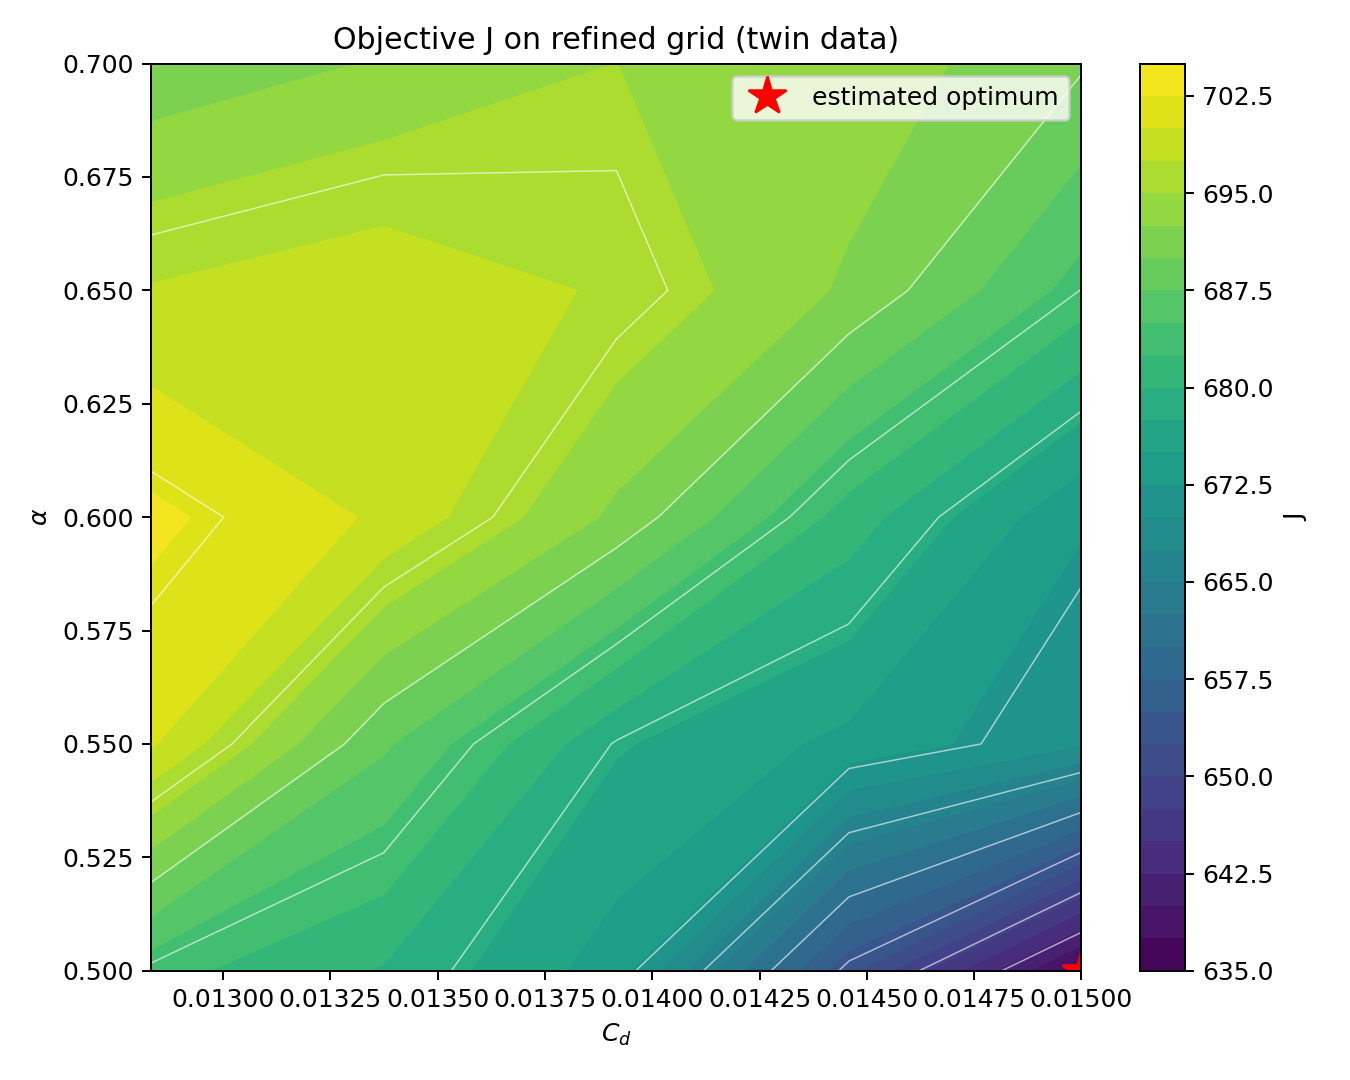
\includegraphics[width=0.76\textwidth]{figures/problem3_objective_contour.png}
\caption{真实观测下 $J(C_d,\alpha)$ 的粗--细网格等高线与最佳已采样边界点}
\label{fig:p3_real_contour}
\end{figure}

\subsection{孪生试验：算法识别精度}

为区分优化器能力与真实数据拟合困难，构造孪生试验：以 $(C_d,\alpha)=(0.008,1.2)$ 的同一 M1 生成合成观测并叠加 $\sigma=0.01\ \mathrm{m/s}$ 高斯噪声。网格搜索恢复为 $(0.00893,1.25)$、$J=6.66$，Nelder--Mead 恢复为 $(0.00812,1.158)$、$J=6.65$，$C_d$ 误差不超过 $0.001$、$\alpha$ 不超过 $0.05$。该结果说明算法在模型一致的合成场景中能够识别参数；真实数据 $J\approx636$ 远大于孪生试验 $J\approx6.7$，提示 M1 结构、边界观测处理或误差模型可能与真实观测生成机制不一致，但不能仅凭孪生试验把全部残差唯一归因于 M1。

\begin{figure}[H]
\centering
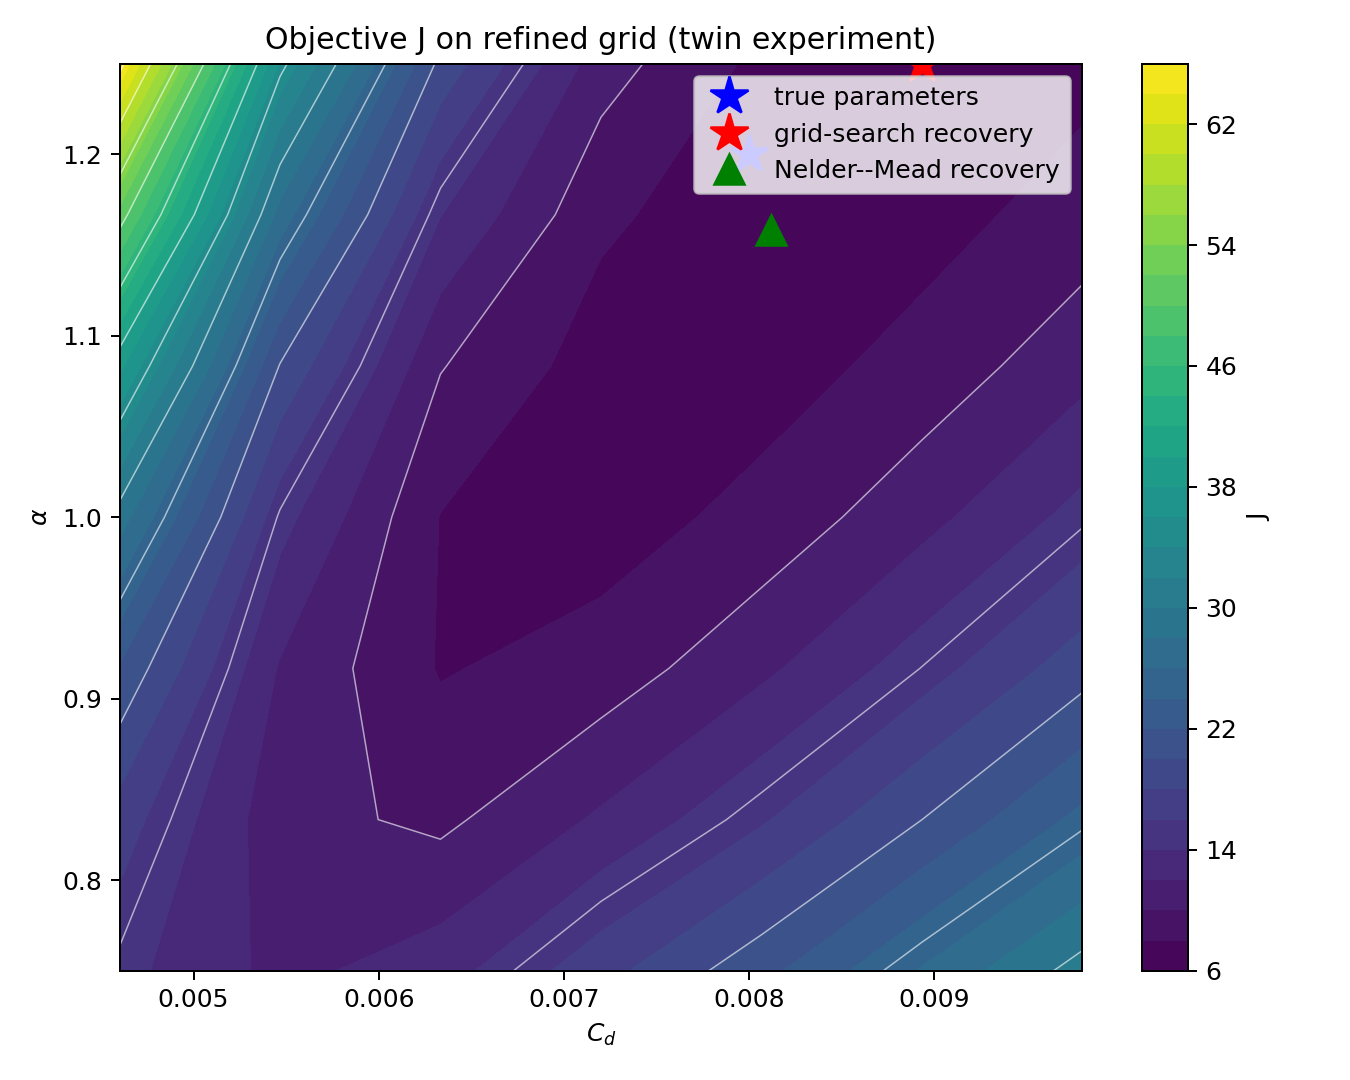
\includegraphics[width=0.72\textwidth]{figures/problem3_twin_contour.png}
\caption{孪生试验中目标函数 $J(C_d,\alpha)$ 细网格等高线（真实参数 $(0.008,1.2)$，网格搜索恢复 $(0.00893,1.25)$）}
\label{fig:p3_contour}
\end{figure}

\subsection{40×20 验证与残差结构分析}

以 $(C_d^*,\alpha^*)=(0.015,0.5)$ 在 $40\times20$ 网格运行 24 h，288 个物理步全部收敛且无需重试。六个站点的观测与模拟见表 \ref{tab:p3_station}。

\begin{table}[H]
\centering
\caption{最佳已发现参数下的站点冰速拟合（单位：m/s）}
\renewcommand{\arraystretch}{1.3}
\begin{tabular*}{\textwidth}{@{\extracolsep{\fill}}ccccc@{}}
\toprule[1pt]
站点 & 观测 $(U,V)$ & 模拟 $(U,V)$ & 残差模 & 权重说明\\
\midrule
1 & $(0.100,0.070)$ & $(0.0607,0.0206)$ & $0.0631$ & 内部点\\
2 & $(0.180,0.080)$ & $(0.0612,0.0222)$ & $0.1321$ & 内部点\\
3 & $(0.110,0.090)$ & $(0.0475,0.0126)$ & $0.0995$ & 内部点\\
4 & $(0.070,0.140)$ & $(0.0440,0.0199)$ & $0.1229$ & 内部点\\
5 & $(0.060,0.120)$ & $(0.0054,0.0012)$ & $0.1307$ & 内部点\\
6 & $(0.040,0.080)$ & $(0,0)$ & $0.0894$ & 固壁点，方差放大\\
\bottomrule[1pt]
\end{tabular*}
\label{tab:p3_station}
\end{table}

内部站点的模拟速度普遍偏低，北向分量的欠估尤为明显；固壁站点 6 的差异则由观测误差模型降低权重。在当前参数域内，调节 $C_d$ 与 $\alpha$ 主要改变速度幅值，难以同时修复所有站点的方向和空间差异。该现象与 M1 删除海冰直接科里奥利响应后可能出现方向偏差的机制相符，但也可能受到边界条件、观测代表性和粗网格插值影响，尚不能作唯一因果归因。因此，反演结果应解释为 M1 条件下的校准候选，而不是对真实物理参数的无偏估计。

\section{问题四：初始冰厚场反演与 48 h 预报}

\subsection{问题分析}

问题四从少量速度观测反推二维初始冰厚场，是一个典型的高维欠定反问题。初始冰厚并不直接被观测，而是先改变冰强度和应力传递，再通过 6--24 h 的动力过程影响站点冰速；这一间接映射会削弱小尺度信息。题定网格包含 20000 个厚度未知量，而可用观测只有 36 个标量分量，逐格反演不仅不可辨识，也会把观测噪声放大为空间振荡。本文因此先用低频谱基提取观测可能约束的大尺度结构，再通过背景项限制修正幅度，最后将所得候选场送入 48 h 正演，考察其动力一致性。

\subsection{病态性与谱参数化降维}

题定网格初始冰厚自由度为 20000，而观测仅 6 个位置、3 个时刻共 18 组向量、36 个标量分量，属严重欠定反问题\cite{tikhonov1977}。本文采用低频谱参数化
\begin{equation}
h_0(x,y)=\operatorname{clip}\left[
h_b(x,y)+\sum_{k=0}^{3}\sum_{l=0}^{2}
c_{kl}\cos\frac{k\pi x}{L_x}\cos\frac{l\pi y}{L_y},\ 0,\ 1.5
\right],
\end{equation}
以 $4\times3=12$ 个低频余弦系数控制全场大尺度修正。余弦基函数满足零法向梯度边界；截断至 $k\le3,l\le2$ 仅允许大尺度修正，本身构成主要空间平滑约束。系数边界与厚度夹逼 $\mathrm{clip}(\cdot,0,1.5)$ 防止非物理厚度，但也使目标函数在触及夹逼点时仅分段光滑。降维牺牲小尺度修正能力，却与当前观测的信息量相匹配。

设 $\mathcal H_{k,t}(\vect c)$ 为以谱系数 $\vect c$ 构造初始场后，前向模型在站点 $k$、时刻 $t$ 输出的冰速，目标函数写为
\begin{equation}
J(\vect c)=
\sum_{k,t}\left\|\mathsf R_{k,t}^{-1/2}
\bigl[\mathcal H_{k,t}(\vect c)-\vect U_{k,t}^{\mathrm{obs}}\bigr]\right\|_2^2
+\lambda_b\|h_0(\vect c)-h_b\|_2^2
+\lambda_s\|\nabla h_0(\vect c)\|_2^2.
\label{eq:p4_obj}
\end{equation}
第一项衡量观测拟合，第二项限制候选场偏离背景场的幅度，第三项用于抑制空间振荡。由于低频谱截断已经提供了强平滑，本文把背景正则化作为主要稳定机制；显式梯度正则项仅在权重实现有效时才可用于敏感性比较。

式 \eqref{eq:p4_obj} 中，$\vect c=(c_{00},\ldots,c_{32})^\mathsf T$ 是 12 维谱系数向量；$\mathcal H_{k,t}$ 表示“由系数生成初始厚度场、完成正演并在站点插值”的复合观测算子；$\mathsf R_{k,t}$ 是观测误差协方差，决定不同站点和速度分量的权重。$h_b$ 为背景初始场，$\lambda_b$ 控制候选场偏离背景的代价，$\lambda_s$ 控制空间梯度惩罚。因而该目标函数并非只追求站点拟合最小，而是在观测一致性、背景可信度和空间平滑性之间折中。

\begin{table}[H]
\centering
\caption{初始场反演候选方法比较}
\renewcommand{\arraystretch}{1.35}
\begin{tabular*}{\textwidth}{@{\extracolsep{\fill}}p{2.5cm}p{3.0cm}p{3.0cm}p{3.1cm}@{}}
\toprule[1pt]
方法 & 优点 & 局限 & 本题适用性\\
\midrule
逐网格优化 & 保留全部空间自由度 & 20000 维严重欠定，梯度和存储代价高 & 不采用\\
集合卡尔曼类 & 可表达背景协方差和不确定性 & 需要大量集合正演，样本协方差易退化 & 适合观测更多、算力更充足的扩展\\
伴随/四维变分 & 高维梯度成本与参数维数近似无关 & 需推导和维护完整伴随模型 & 可作为后续高精度方案\\
低频谱 + L-BFGS-B & 维数低、边界约束方便、易并行差分 & 难恢复小尺度结构，仍依赖正演预算 & 与 36 个标量观测和竞赛算力匹配\\
\bottomrule[1pt]
\end{tabular*}
\label{tab:p4_method_compare}
\end{table}

\subsection{算法选择与理由}

在 12 维昂贵正演问题中，穷举或进化算法的求值成本过高；L-BFGS-B 原生支持系数边界，并可用有限差分近似梯度，作为低维、带界、分段光滑问题的候选优化器是合理的\cite{liu1989,nocedal2006}。实现采用 12 个方向的并行前向差分，而非解析梯度或中心差分。由于夹逼操作和数值正演会降低光滑性，L-BFGS-B 的收敛状态必须作为结果的一部分检查，不能仅凭目标下降宣称得到最优解。

\subsection{预算内优化结果与正则化证据边界}

程序设置 $\kappa_s=0$ 与 $0.5$ 两档进行试算，两次 L-BFGS-B 均在 10 次迭代、20 次目标评估后达到预算上限。进一步检查发现，$\lambda_s$ 按当前场梯度能量的倒数动态缩放，使 $\lambda_s\sum|\nabla h|^2$ 近似保持常数，因而没有向优化器提供有效的平滑梯度。故两档结果不能被解释为正规的平滑参数敏感性试验；本问真正发挥稳定作用的是低频谱截断和背景正则化。

\begin{table}[H]
\centering
\caption{L-BFGS-B 预算受限候选结果}
\renewcommand{\arraystretch}{1.4}
\begin{tabular*}{\textwidth}{
    @{\extracolsep{\fill}}
    l
    c
    c
    c
    c
    c
    @{}
}
\toprule[1pt]
$\kappa_s$ & 候选 J & 背景 J & J 下降 & $\max|h_0-h_b|$/m & 收敛状态\\
\midrule
$0$ & $1037.7$ & $1072.2$ & $3.22\%$ & $0.0379$ & 达迭代上限\\
$0.5$ & $6487.7$ & $6522.2$ & $0.53\%$ & $0.0379$ & 达迭代上限\\
\bottomrule[1pt]
\end{tabular*}
\label{tab:p4_sens}
\end{table}

可可靠陈述的结果是：在 $\kappa_s=0$ 的定义良好目标下，预算内候选使总正则化目标由 $1072.2$ 降至 $1037.7$（$3.22\%$），最大厚度修正为 $0.0379\ \mathrm m$。保存文件未分离候选点的观测残差项与背景惩罚项，故不能把 $3.22\%$ 全部解释为观测拟合改善；两档保存的“predicted velocity RMS”是预测速度幅值 RMS，也不是观测残差 RMS。$\kappa_s=0.5$ 的总目标因加入近似常数而与 $\kappa_s=0$ 不可横向比较。由此本文把 $\kappa_s=0$ 结果称为预算受限低频正则化候选，不称为收敛最优解。

\subsection{48 h 预报结果}

以该候选初始场为初值，在 $40\times20$ 网格上运行 48 h（576 步，全部收敛、冰体积机器精度守恒），结果见表 \ref{tab:p4_48h} 与图 \ref{fig:p4_48h}。该运行验证候选场能够稳定进入正演并产生守恒预报，不证明反演候选已经优化收敛。

\begin{table}[H]
\centering
\caption{40×20 网格候选初始场的 48 h 正演统计}
\renewcommand{\arraystretch}{1.4}
\begin{tabular*}{\textwidth}{
    @{\extracolsep{\fill}}
    l
    c
    @{}
}
\toprule[1pt]
指标 & 数值\\
\midrule
48 h 平均冰厚 / m & $0.484178$\\
48 h 最大冰速 / (m/s) & $0.107166$\\
48 h 中心点冰厚 / m & $0.809516$\\
冰体积相对误差 & $0$（机器精度）\\
最小/最大冰厚 / m & $2.6\times10^{-8}$ / $0.939823$\\
\bottomrule[1pt]
\end{tabular*}
\label{tab:p4_48h}
\end{table}

48 h 正演中，区域平均冰厚 $0.484178\ \mathrm m$ 在闭域零通量下保持机器精度守恒；全域最大冰速为 $0.107166\ \mathrm{m/s}$，中心点冰厚为 $0.809516\ \mathrm m$。图 \ref{fig:p4_48h} 中候选初始场与背景场接近（最大偏差 3.8 cm），48 h 冰厚场的大尺度结构也相近。该结果说明低频小扰动候选不会破坏正演稳定性，但不能由此判断其观测拟合优于其他未搜索场。

\begin{figure}[H]
\centering
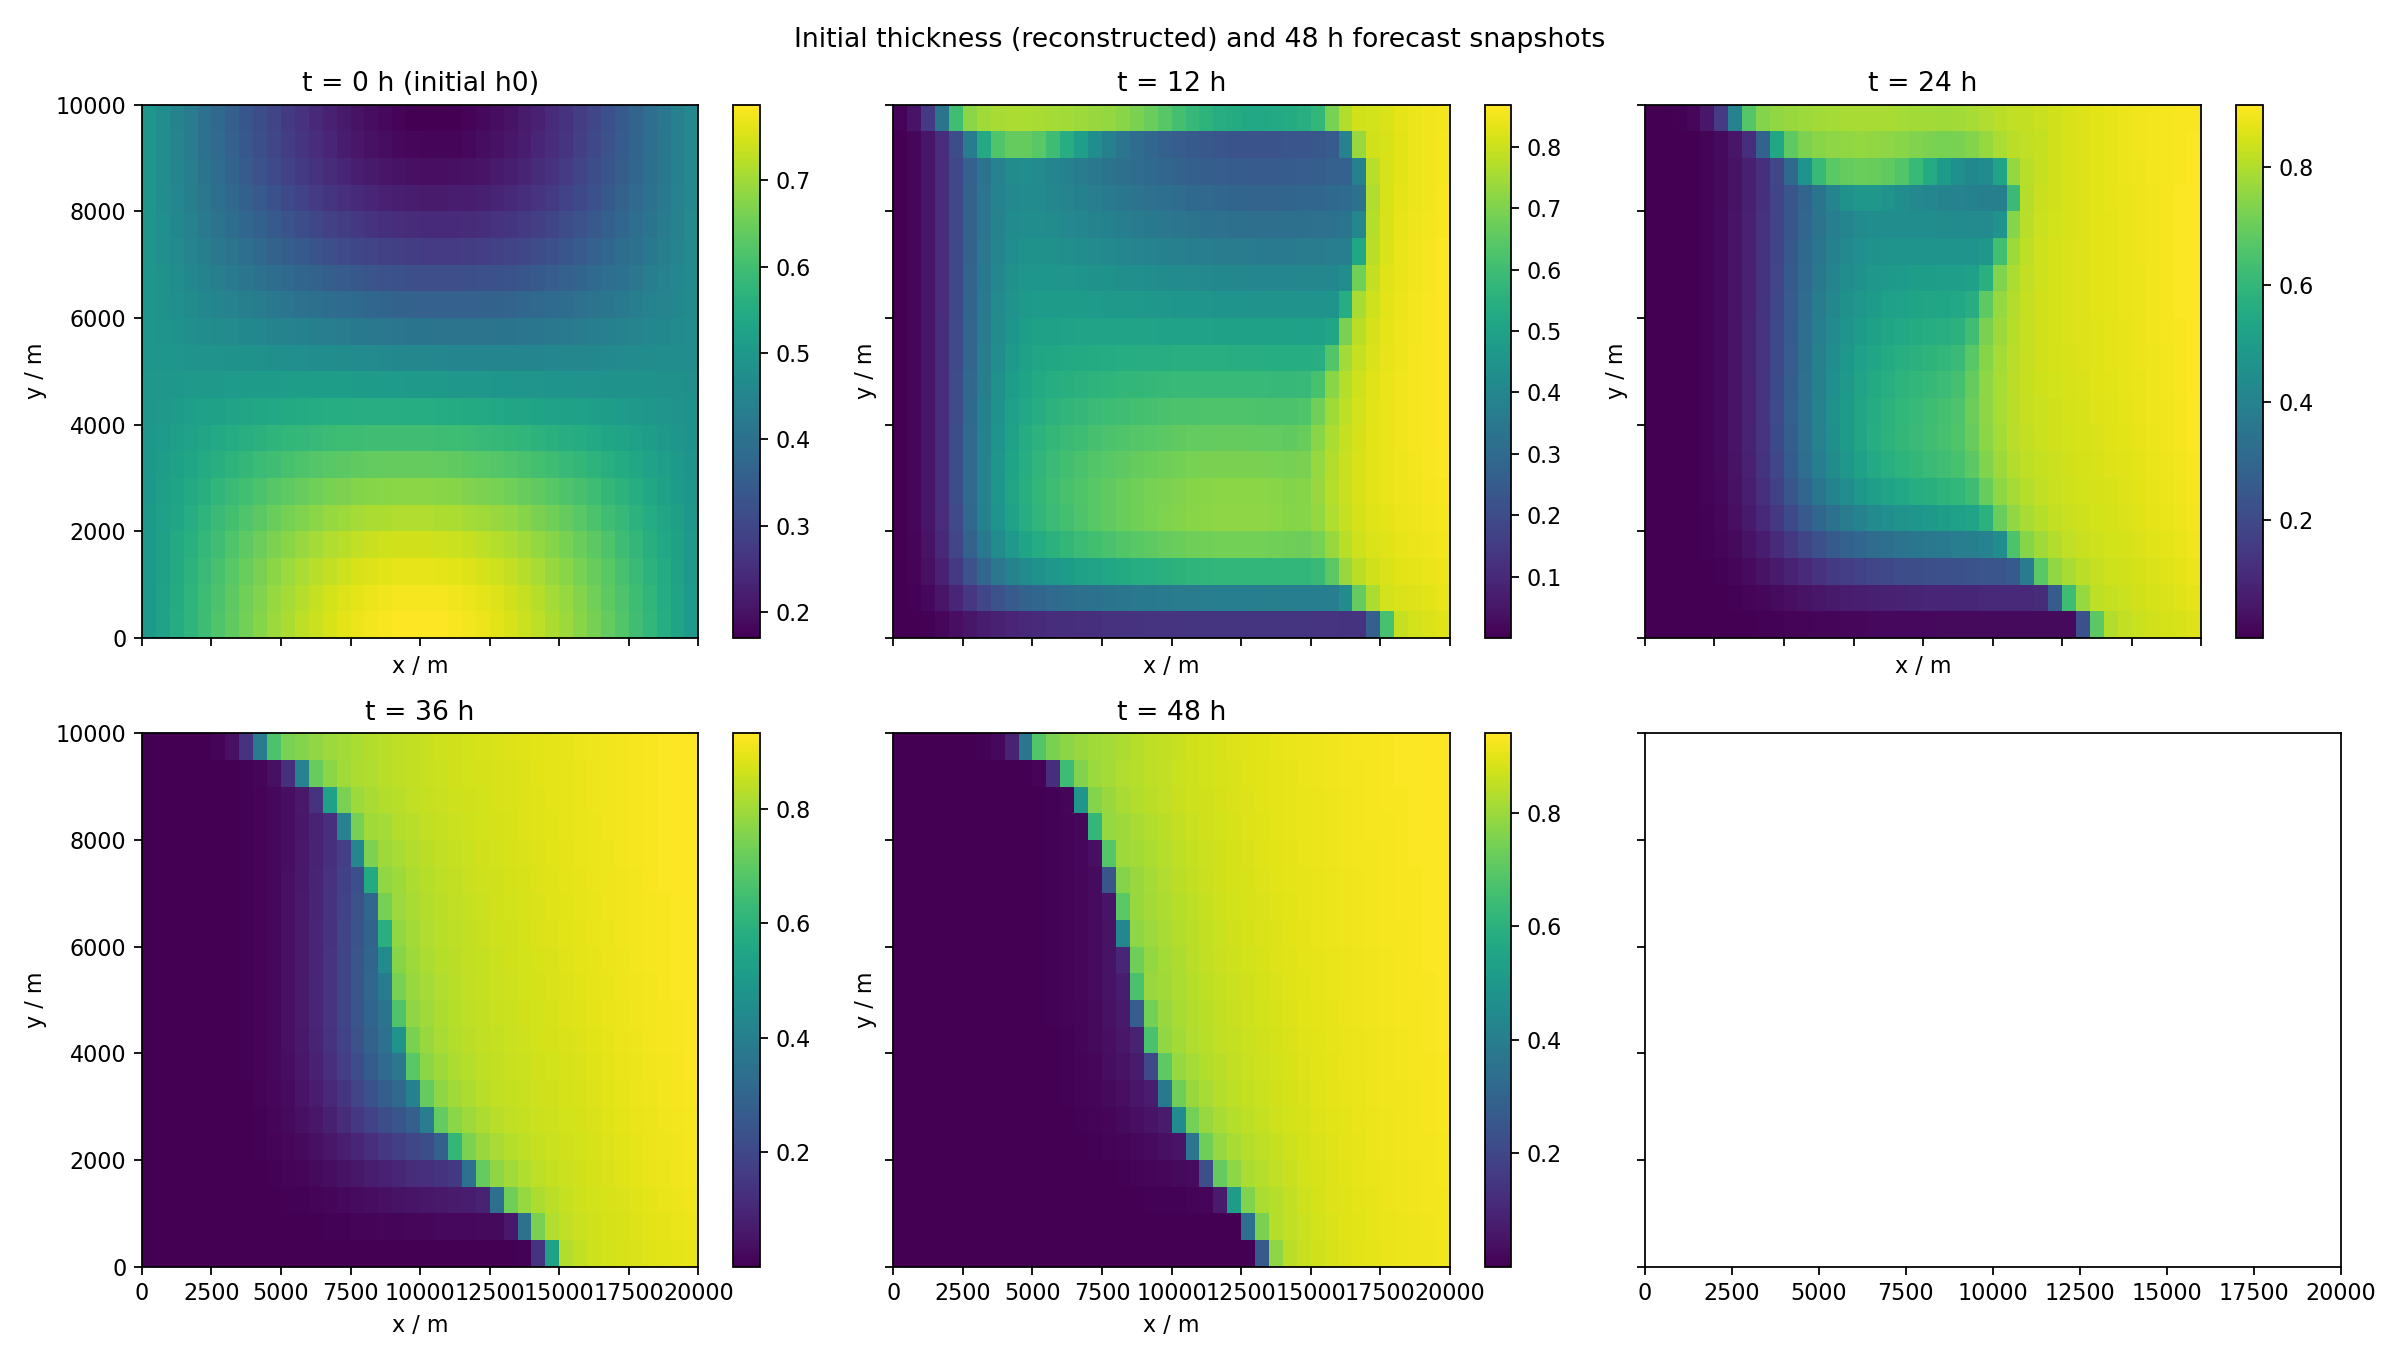
\includegraphics[width=0.95\textwidth]{figures/problem4_thickness_snapshots_48h.png}
\caption{候选初始冰厚场与 48 h 冰厚正演}
\label{fig:p4_48h}
\end{figure}

图 \ref{fig:p4_velocity} 给出 48 h 冰速场。较大冰速集中在西南侧薄冰和冰缘区域，厚冰主体内部速度较低，整体方向与东向风应力、海水拖曳及 VP 内力共同作用下的结果相容。该空间格局与问题二 24 h 结果相近，且未出现新的孤立高速斑块；但由于候选场只包含低频修正，图中的平滑结构也反映了谱截断对小尺度变化的抑制。这里的比较属于场形态检查，不替代逐点力预算或预报精度验证。

\begin{figure}[H]
\centering
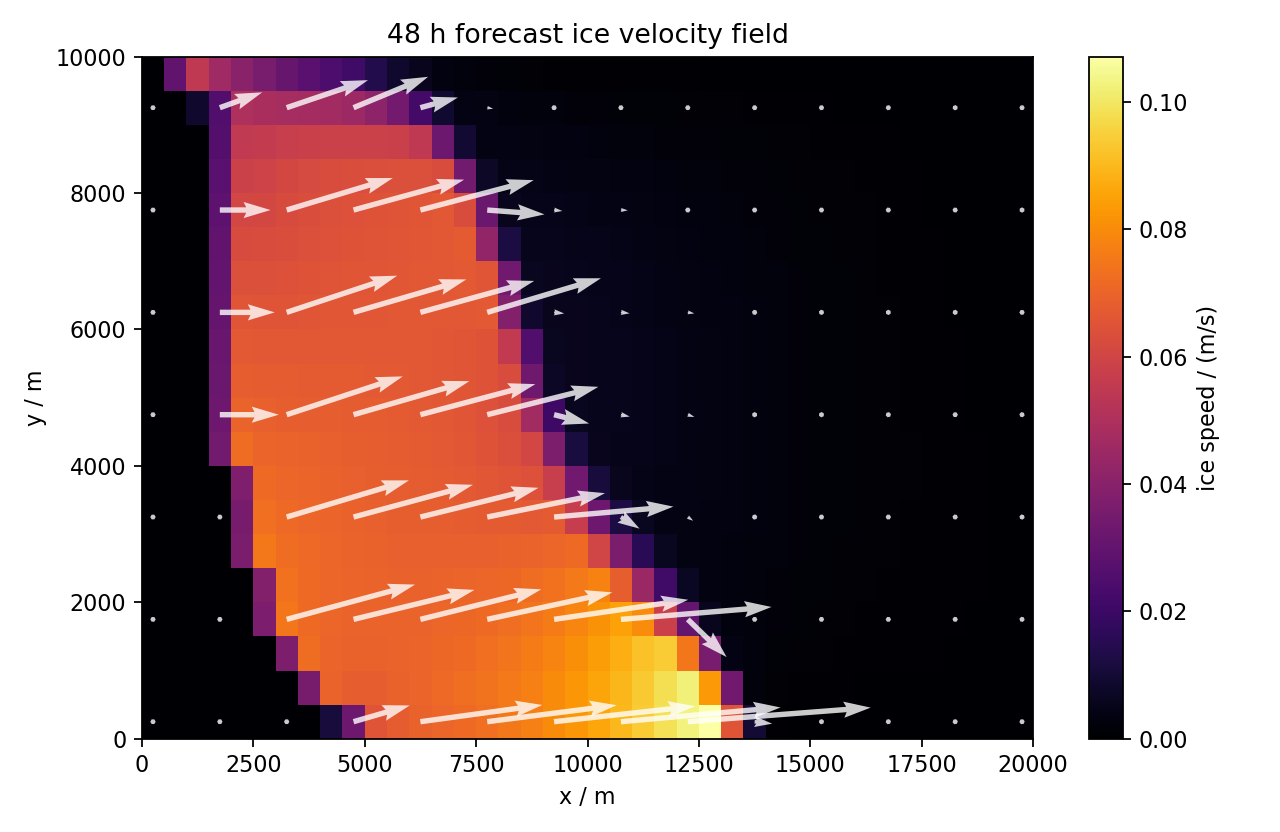
\includegraphics[width=0.80\textwidth]{figures/problem4_velocity_field_48h.png}
\caption{候选初始场驱动的 48 h 海冰速度分布}
\label{fig:p4_velocity}
\end{figure}

\section{问题五：时变冰情下 LNG 船航线优化}

\subsection{问题分析}

问题五把连续的海冰预报场转化为船舶可执行的航行决策。冰密集度同时影响两类约束：当 $A>0.6$ 时航段不可通行；在允许通行的区域内，$A$ 越大，船速越低、单位航程所需时间和燃油也随之改变。由于冰场在航行过程中继续演化，某一空间格是否可通行以及穿越它的代价都依赖到达时刻，因此不能把 24 h 冰场简单冻结为静态地图。本文先对题设终点进行全时段可行性检查，再在时间分层路网上搜索燃油最小路径，并以静态冰场方案衡量使用预报信息带来的边际收益。

\subsection{模型与离散}

以 $(C_d^*,\alpha^*)=(0.015,0.5)$ 与初始场候选运行 M1，生成 $t\in[24,72]\ \mathrm h$ 逐小时冰密集度场（40×20 网格、864/864 步收敛、体积守恒）。LNG 船最大航速 $V_{\max}=15\ \mathrm{kt}=7.716\ \mathrm{m/s}$，$A>0.6$ 禁行，可通行区航速 $V_s=V_{\max}(1-A)$，油耗率 $q=q_0+q_1V_s^2$，其中 $q_0=0.5\ \mathrm{t/h}$；若 $V_s$ 以 $\mathrm{m/s}$ 计，则 $q_1$ 的量纲应写作 $(\mathrm{t/h})/(\mathrm{m/s})^2$。空间节点取 40×20 网格中心，起点 S 离散到最近中心 $(750,4750)$；时间层 $\Delta\tau=5\ \mathrm{min}$，边含 8 邻域移动和原地等待。移动耗时按距离/航速计算，禁行判定检查出发、中点与到达位置。

设航段 $e$ 的长度为 $d_e$，进入该段时刻为 $t_e$，沿段插值得到的代表冰密集度为 $A_e(t_e)$，则
\begin{equation}
\Delta t_e=\frac{d_e}{V_{\max}[1-A_e(t_e)]},
\qquad
\Delta Q_e=\left\{q_0+q_1V_{\max}^2[1-A_e(t_e)]^2\right\}\Delta t_e.
\end{equation}
其中，$d_e$ 是相邻路网节点间的几何距离，$t_e$ 是船舶进入航段 $e$ 的时刻，$A_e(t_e)$ 是沿航段进行时空插值得到的代表冰密集度。$\Delta t_e$ 为通过该航段所需时间，$\Delta Q_e$ 为相应燃油消耗；$q_0$ 表示与航速无关的基础耗油率，$q_1$ 则描述航速升高引起的附加耗油。由于 $A_e$ 同时进入分母中的航速和油耗率，密集度升高会延长航时，但对单段燃油的净影响还取决于基础耗油与速度平方项的相对大小。
路径 $P$ 的优化模型为
\begin{align}
\min_P\quad &Q(P)=\sum_{e\in P}\Delta Q_e,\\
\text{s.t.}\quad
&A_e(t_e)\le0.6,\qquad t_e+\Delta t_e\le72\ \mathrm h,\\
&e\text{ 满足 8 邻域移动或等待规则，且路径连续。}
\end{align}
等待边允许船舶在局部冰情改善时延后进入某一区域。由于所有燃油增量非负，最短路标签具有单调增加性质，为 Dijkstra 类算法提供了基础。

\subsection{算法选择与理由}

非负燃油边权使 Dijkstra 成为合理的图搜索基线\cite{dijkstra1959,cooke1966}，并比遗传/粒子群更容易维持禁行约束。严格的时空展开图需要把每个精确到达时刻作为独立状态，或满足 FIFO 条件后使用相应时变最短路算法；当前实现用 $(\text{空间格},\lfloor t/\Delta\tau\rfloor)$ 编号，并在同一时间层只保留一组燃油--到达时刻标签，而后续边权又依赖精确时刻。因此标签压缩可能丢弃对未来更有利的状态，经典 Dijkstra 全局最优性不能直接套用。本文将其定位为\textbf{时间分层 Dijkstra 近似搜索}，并以静态场和两档时间层作经验对照。

\begin{table}[H]
\centering
\caption{航线规划方法比较}
\renewcommand{\arraystretch}{1.35}
\begin{tabular*}{\textwidth}{@{\extracolsep{\fill}}p{2.6cm}p{3.1cm}p{3.0cm}p{3.0cm}@{}}
\toprule[1pt]
方法 & 优点 & 局限 & 本文定位\\
\midrule
静态 Dijkstra/A* & 速度快、最优性条件清楚 & 忽略航行期间冰情变化 & 冻结 24 h 冰场的基准\\
遗传算法/粒子群 & 可处理连续航迹和复合目标 & 禁行约束修复困难，随机性强 & 不作为主算法\\
严格时空展开图 & 保留到达时刻，可给出离散全局最优 & 状态数随时间层数快速增加 & 理论上最完整的改进方向\\
时间分层 Dijkstra & 计算量可控，禁行约束显式 & 单标签压缩削弱严格最优保证 & 本文候选路线求解器\\
\bottomrule[1pt]
\end{tabular*}
\label{tab:p5_method_compare}
\end{table}

\subsection{对比实验：时变场与静态场}

将时变 Dijkstra 与“以 t=24 h 冰场冻结”的静态方案对照（表 \ref{tab:p5_route}），并做时间离散敏感性（$\Delta\tau=5$ 与 10 min）。

\begin{table}[H]
\centering
\caption{航线优化结果对比}
\renewcommand{\arraystretch}{1.4}
\begin{tabular*}{\textwidth}{
    @{\extracolsep{\fill}}
    l
    c
    c
    c
    c
    @{}
}
\toprule[1pt]
方案 & 总燃油/t & 总航时/h & 到达时刻/h & 说明\\
\midrule
时变 Dijkstra（5 min） & $0.484026$ & $0.6179$ & $24.62$ & 放宽问题候选\\
时变 Dijkstra（10 min） & $0.484026$ & $0.6179$ & $24.62$ & 离散敏感性（一致）\\
静态 t=24 h 场（5 min） & $0.484636$ & $0.6193$ & $24.62$ & 对照方案\\
\bottomrule[1pt]
\end{tabular*}
\label{tab:p5_route}
\end{table}

表 \ref{tab:p5_route} 表明：在同一放宽终点下，5 min 时变候选比 t=24 h 静态候选少耗油约 $0.13\%$、少航时约 $0.2\%$，收益在本场景中很小；5 min 与 10 min 输出在报告精度内相同，说明候选路线对这两档时间层不敏感，但不能排除更细时间离散或标签压缩误差。时变/静态的差异可作为当前预报场下时变信息的边际收益，不能外推为快速演变场景中必然显著优越。

\begin{figure}[H]
\centering
\begin{minipage}[t]{0.49\textwidth}
\centering
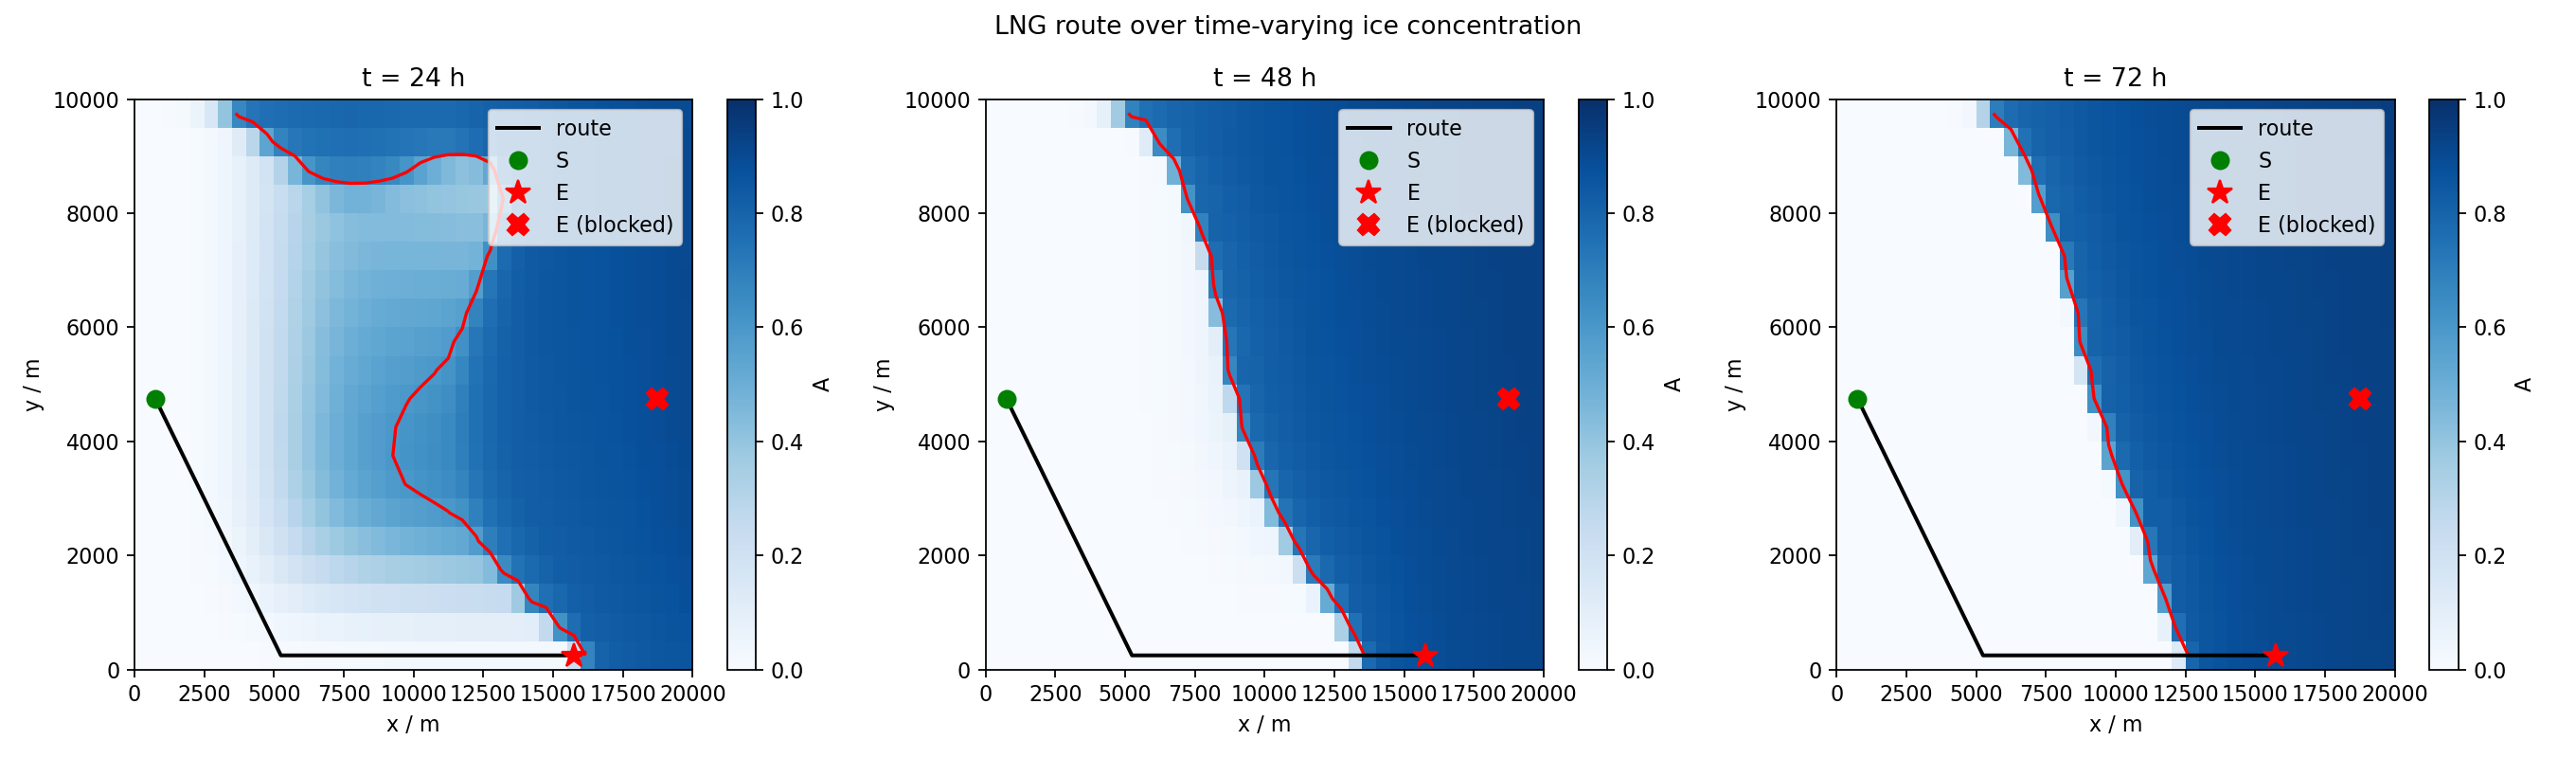
\includegraphics[width=\textwidth]{figures/problem5_route_tau5.png}\\
{\small (a) 时变冰场候选路线}
\end{minipage}
\hfill
\begin{minipage}[t]{0.49\textwidth}
\centering
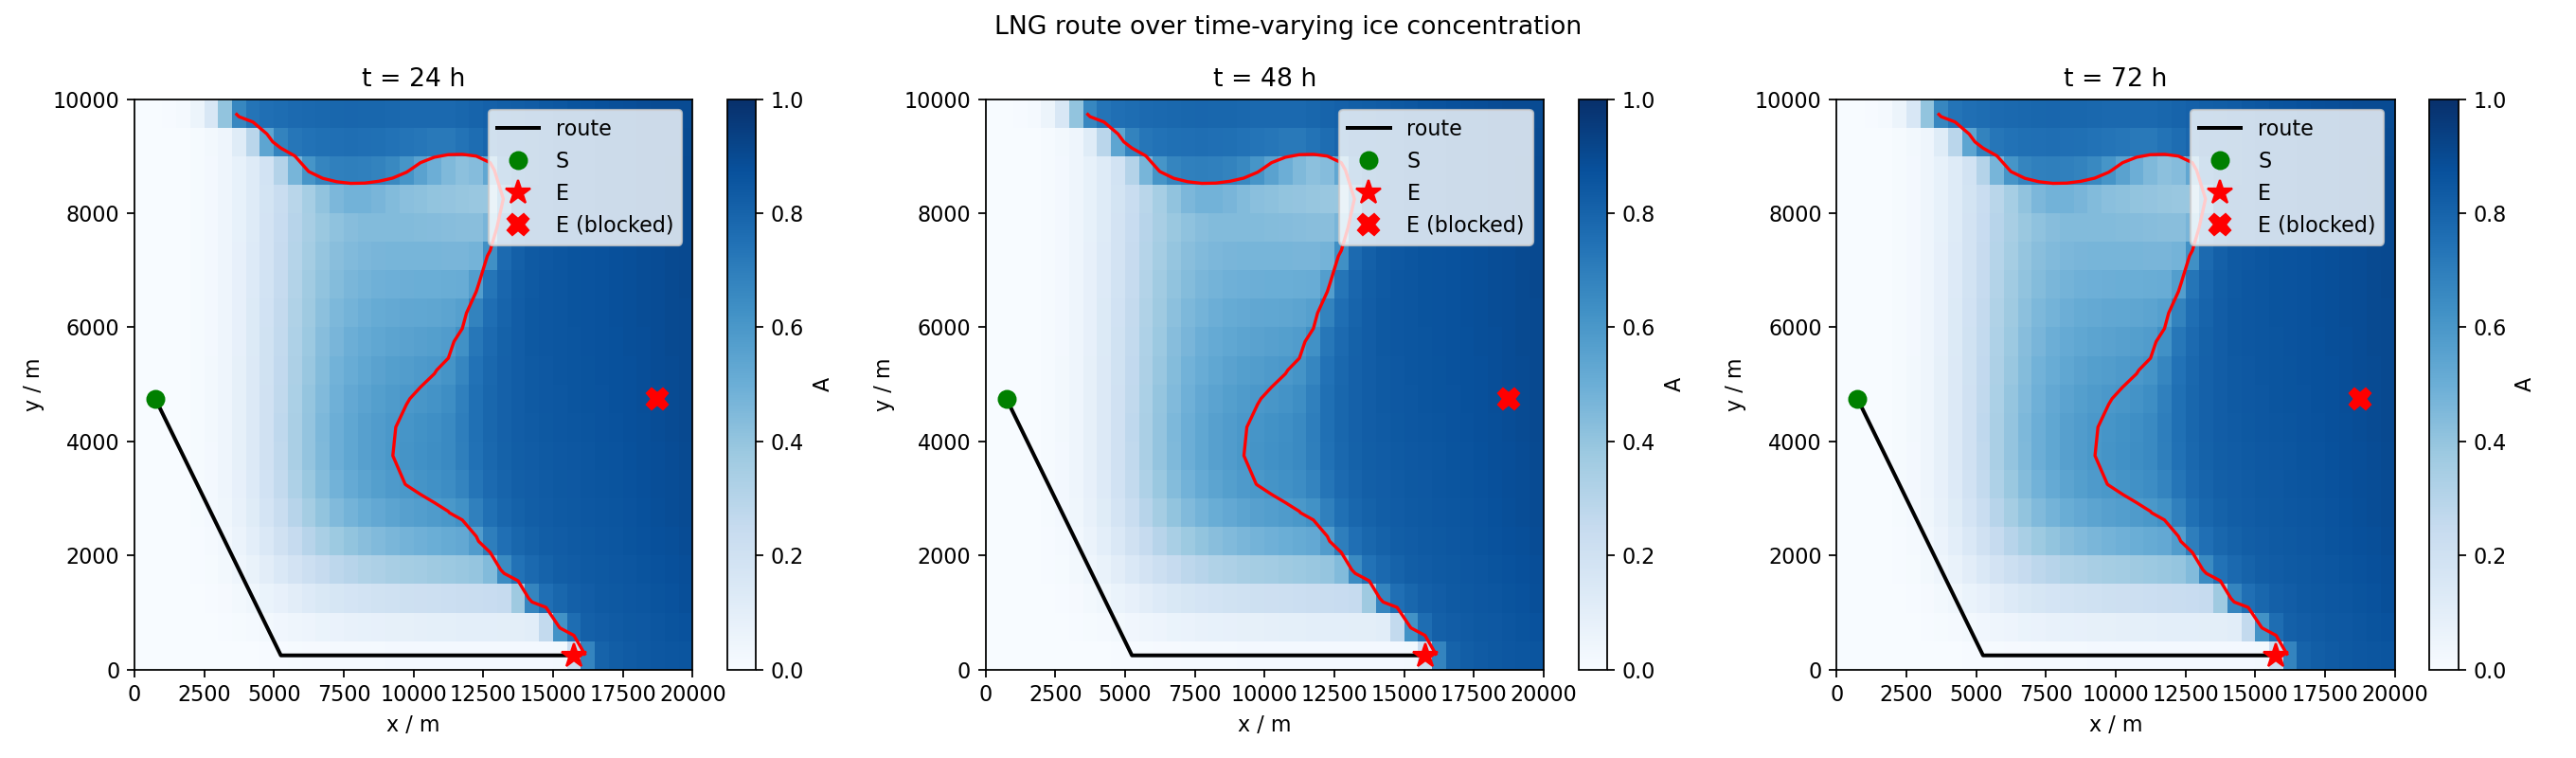
\includegraphics[width=\textwidth]{figures/problem5_route_static_24h.png}\\
{\small (b) 冻结 24 h 冰场候选路线}
\end{minipage}
\caption{时变方案与静态方案的航迹对比}
\label{fig:p5_compare}
\end{figure}

\subsection{严格不可行判定与放宽终点候选路线}

在 M1 预报中，终点 E 的最近网格中心 $(18750,4750)$ 在 24--72 h 的冰密集度始终位于 $0.890$--$0.931$，明显高于禁行阈值，故原问题在该预报情景下无可行解。为给出具有工程参考意义的备选方案，本文另行选择 t=24 h 时距 E 最近的可通行格 $(15750,250)$ 作为接驳点。按连续坐标题设终点计算，接驳点偏离约 $5.76\ \mathrm{km}$；若以终点对应的最近网格中心 $(18750,4750)$ 为离散比较对象，偏离约 $5.408\ \mathrm{km}$。候选路线从离散起点向西南进入低密集度走廊，再沿南侧开阔水域向东航行，31 个航路点均满足 $A\le0.6$。这一结果适用于“船舶抵达接驳点、后续改用破冰或陆岸转运”的放宽场景，不能替代题设终点的严格到达方案。

时变方案仅比静态方案节油 $0.13\%$，并不意味着逐小时预报没有价值。本例候选航迹主要穿过低密集度南部走廊，且总航时不足 1 h，航行期间冰场变化很小，因而两种方案自然接近；若航程更长、等待行为更频繁或禁行边界移动更快，静态近似的代价才可能显著增加。

\section{模型评价、灵敏度分析与推广}

\subsection{模型优点}

\begin{enumerate}
\item \textbf{物理结构前后一致：}问题一至问题五共用厚度加权 VP 内力、同一冰水拖曳定义和相同边界条件，参数反演与航线规划建立在同一前向模型上，减少了不同章节之间的物理口径冲突；
\item \textbf{兼顾稳定性与计算效率：}C 型网格、IMEX 浅水推进和守恒冰厚输运分别针对压力振荡、重力波 CFL 和质量守恒问题；受保护 Anderson 与 ILU 复用在保持离散固定点近似不变的同时降低了长时程计算成本；
\item \textbf{模型选择具有对照依据：}问题一通过单删项实验解释双删项差异的来源，问题三用三种优化算法和孪生试验检查参数可辨识性，问题五用静态冰场方案衡量时变预报的实际收益；
\item \textbf{能够报告不可行与负结果：}当 M1 结构差异超过参考线、初始场优化未收敛或题设终点不可通行时，模型不强行给出“通过”结论，而是将这些结果用于界定适用范围和提出工程备选方案。
\end{enumerate}

\subsection{稳健性与局限性}

主要局限包括：题定 $200\times100$ 网格的 24 h 全时段尚未完成，$100\times50$ 结果只能作为可完成替代网格；M1 与同离散完整模型的结构差异在当前场景中达到 $7.8\%$--$13.4\%$，该差异会向参数反演和航线规划传播；问题三的最佳已发现参数位于搜索边界，说明参数域或模型结构仍可能限制拟合；问题四受正演预算约束，L-BFGS-B 在迭代上限处停止，且现有显式平滑权重没有形成有效梯度；问题五采用单标签时间压缩，所得路线是离散候选而非严格时空全局最优。

\subsection{误差传播与适用情景}

本题的五个问题构成串联系统，上游误差会改变下游最优解的含义。表 \ref{tab:error_propagation} 总结主要不确定性及其影响。

\begin{table}[H]
\centering
\caption{主要误差来源及其向下游的传播}
\renewcommand{\arraystretch}{1.35}
\begin{tabular*}{\textwidth}{@{\extracolsep{\fill}}p{2.5cm}p{3.4cm}p{3.4cm}p{2.7cm}@{}}
\toprule[1pt]
来源 & 直接影响 & 下游表现 & 论文中的处理\\
\midrule
M1 双删项 & 冰速方向和调整过程偏差 & 参数可能吸收结构误差，航线禁行区位置改变 & M0/$M_I$/$M_C$ 对照与 A--D 归因\\
空间网格不足 & 冰缘和速度极值位置偏移 & 站点插值及路径可通行格发生变化 & 40×20 与 100×50 统计一致性比较\\
观测误差与代表性 & 参数目标函数增大 & 边界参数、站点残差不均匀 & 方差加权和固壁点降权\\
初始场降维 & 小尺度厚度结构无法恢复 & 48 h 冰缘较平滑、局部风险可能低估 & 明确限制为低频候选场\\
时间层与标签压缩 & 丢失部分到达时刻状态 & 路线燃油和等待策略存在离散误差 & 5/10 min 对照并保留最优性限制\\
\bottomrule[1pt]
\end{tabular*}
\label{tab:error_propagation}
\end{table}

因此，本文模型更适合用于缓变边缘冰区中的方案比较、参数敏感性研究和短时航线候选生成。对于快速风场突变、离散碎冰碰撞、厚冰强挤压带或必须保证严格到达的高风险航次，应保留完整海冰动力、采用更细网格和集合预报，并将航线规划改写为考虑预报不确定性的鲁棒或机会约束模型。

\subsection{灵敏度分析}

稳健性检验覆盖四个维度：时间步由 $300$ s 与 $150$ s 对照；求解器由 24 h 优化前后固定点差异和 6 h 直接/迭代线性求解对照；参数识别由三算法比较与模型一致孪生试验；航线离散由 5 min 与 10 min 时间层对照。结果显示，收紧残差几乎不改变 M1--M0 结构差异，求解器优化后的场差异最大为 $0.0228\%$，两档航线时间层输出在报告精度内一致。$\kappa_s=0/0.5$ 因平滑项近似常数，不作为有效灵敏度证据。

\subsection{改进方向}

可扩展方向包括：完成题定 $200\times100$ 全时段并进行至少三层网格收敛研究；将稀疏直接 LU 的 6 h 优势扩展到 24 h 与更高网格验证；修复显式平滑权重并重新运行收敛的初始场反演，或用伴随梯度降低成本；把航线状态改为严格时空展开、多标签 Dijkstra 或满足 FIFO 的时变最短路，并在严格终点不可行时显式加入破冰船接驳或终点偏差惩罚。

\section{结论}

\subsection{主要成果总结}

本文完成了北极边缘冰区海冰演化与船舶安全航行的全链条建模，五个问题的结论如下：

\par \textbf{问题一}完成海冰动量方程的量纲订正，将内力统一为厚度加权应力通量散度 $\nabla\cdot(h_i\vect\sigma)$；在题目指定尺度下，惯性力与海冰科里奥利力的合计量级约为三项保留力合计量级的 $4.5636\%$，由此建立瞬时三力平衡 M1。单删项实验表明海冰科里奥利作用对速度方向和冰厚输运影响更明显；严格 D 组中 M1 相对 M0 的四项结构差异为 $7.778\%$--$13.444\%$，而求解残差与时间步敏感性远小于该差异，说明 M1 的适用边界主要由物理删项而非数值容差决定。

\par \textbf{问题二}实现了 C 型交错网格上的冰水耦合求解，并以时间预测、Anderson 和 ILU 复用优化正式 24 h GMRES/ILU 路线。优化后的加速比为 $1.275$，时空场差异最大为 $0.0228\%$。

$100\times50$ 替代网格给出平均冰厚 $0.500000\ \mathrm m$、终时单元中心重构最大冰速 $0.208846\ \mathrm{m/s}$；288 个物理步最终全部接受，其中 113 步经过保护性重试。该运行满足残差、CFL、非负性与冰量守恒检查，但题定 $200\times100$ 全时段尚未完成。

\par \textbf{问题三}三种算法在有限预算下比较：网格搜索与差分进化均指向已采样最佳边界点 $(0.015,0.5)$、$J=636.2$，Nelder--Mead 与差分进化均因预算上限停止。孪生试验仅证明模型一致合成数据下的可辨识性；真实数据大残差提示模型、边界观测或误差模型存在不一致。

\par \textbf{问题四}以低频余弦谱参数化和背景正则化处理 18 组向量观测约束 20000 自由度的欠定问题。L-BFGS-B 在迭代上限处停止，所得仅为预算受限候选；$\kappa_s=0$ 总目标下降 $3.22\%$，最大厚度修正 $0.038\ \mathrm m$。48 h 正演守恒稳定，但不证明反演收敛。

\par \textbf{问题五}M1 预报下题设终点持续禁行，严格抵达问题无可行解。对放宽到 t=24 h 最近可通行格的问题，时间分层 Dijkstra 得到燃油 $0.484026\ \mathrm t$、航时 $0.6179\ \mathrm h$ 的候选路线，较静态候选节省约 $0.13\%$；单标签压缩使其不具备严格全局最优保证。

\subsection{模型特色}

本文的主要特色是把物理简化、数值求解、反问题和航线决策组织在同一海冰--海水前向内核上。每一次方法选择都设置了对应的比较对象：删项用完整模型与单删项模型解释，求解器用固定点等价和重复计时评价，参数反演用不同优化算法与孪生试验交叉检查，航线则先判断严格可行性再比较时变与静态方案。由此，论文不仅给出数值结果，也说明这些结果在什么条件下成立、哪些结论仍受计算预算和模型结构限制。

\subsection{局限性与展望}

主要局限为：题定 $200\times100$ 网格未完成；M1 结构差异超过 $5\%$；参数候选位于边界且算法预算有限；初始场优化未收敛、显式平滑实现无效；航线严格终点不可行且图搜索为单标签近似。未来工作应优先补齐这些证据缺口，再扩展多船协同与随机冰情鲁棒规划。

\section*{AI 工具使用说明}

根据竞赛 AI 工具使用管理规定，本文在程序框架整理、LaTeX 结构调整和文字润色环节使用了 AI 工具辅助，相关工具列入参考文献\cite{openai_codex}，具体用途与人工复核方式见附录 B。本文全部数值均由本地程序运行产生并经人工核验；AI 仅提供结构和表达建议，模型判断、结果解释与正文定稿均由参赛队员完成。

\begin{thebibliography}{99}
\bibitem{yan2026} Yan Y, Wang X, Lin Z, Ren L, Hou Q, Xu Y. Spatiotemporal patterns of maritime incidents along the Northern Sea Route: A 20-year analysis[J]. Ocean \& Coastal Management, 2026, 278: 108220. DOI: 10.1016/j.ocecoaman.2026.108220.
\bibitem{hibler1979} Hibler W D. A dynamic thermodynamic sea ice model[J]. Journal of Physical Oceanography, 1979, 9(4): 815--846.
\bibitem{feltham2008} Feltham D L. Sea ice rheology[J]. Annual Review of Fluid Mechanics, 2008, 40: 91--112.
\bibitem{lepparanta2011} Leppäranta M. The Drift of Sea Ice[M]. 2nd ed. Berlin: Springer, 2011.
\bibitem{zhang1997} Zhang J, Hibler W D. On an efficient and accurate model for sea ice dynamics[J]. Journal of Geophysical Research, 1997, 102(C4): 8691--8710.
\bibitem{saad2003} Saad Y. Iterative Methods for Sparse Linear Systems[M]. 2nd ed. Philadelphia: SIAM, 2003.
\bibitem{hunke1997} Hunke E C, Dukowicz J K. An elastic--viscous--plastic model for sea ice dynamics[J]. Journal of Physical Oceanography, 1997, 27(9): 1849--1867.
\bibitem{arakawa1977} Arakawa A, Lamb V R. Computational design of the basic dynamical processes of the UCLA general circulation model[J]. Methods in Computational Physics, 1977, 17: 173--265.
\bibitem{ascher1997} Ascher U M, Ruuth S J, Spiteri R J. Implicit-explicit Runge--Kutta methods for time-dependent partial differential equations[J]. Applied Numerical Mathematics, 1997, 25(2--3): 151--167.
\bibitem{walker2011} Walker H F, Ni P. Anderson acceleration for fixed-point iterations[J]. SIAM Journal on Numerical Analysis, 2011, 49(4): 1715--1735.
\bibitem{nelder1965} Nelder J A, Mead R. A simplex method for function minimization[J]. The Computer Journal, 1965, 7(4): 308--313.
\bibitem{storn1997} Storn R, Price K. Differential evolution--a simple and efficient heuristic for global optimization over continuous spaces[J]. Journal of Global Optimization, 1997, 11(4): 341--359.
\bibitem{tikhonov1977} Tikhonov A N, Arsenin V Y. Solutions of Ill-Posed Problems[M]. Washington: Winston \& Sons, 1977.
\bibitem{liu1989} Liu D C, Nocedal J. On the limited memory BFGS method for large scale optimization[J]. Mathematical Programming, 1989, 45(1): 503--528.
\bibitem{nocedal2006} Nocedal J, Wright S J. Numerical Optimization[M]. 2nd ed. New York: Springer, 2006.
\bibitem{dijkstra1959} Dijkstra E W. A note on two problems in connexion with graphs[J]. Numerische Mathematik, 1959, 1: 269--271.
\bibitem{cooke1966} Cooke K L, Halsey E. The shortest route through a network with time-dependent internodal transit times[J]. Journal of Mathematical Analysis and Applications, 1966, 14(3): 493--498.
\bibitem{openai_codex} OpenAI Codex/ChatGPT，GPT-5 系列，OpenAI，2026-08．
\end{thebibliography}

\newpage
\appendix
\section*{附录 A：数值验证细节}

附录 A 汇总各环节数值验证：问题二求解器优化前后残差、守恒、正性、CFL 与源码哈希检查全部通过；$100\times50$ 运行的 288 个物理步最终全部接受，其中 113 步经保护性重试、累计 120 次额外尝试，最大冰残差 $9.98\times10^{-4}$、最大耦合残差 $9.998\times10^{-6}$，冰体积相对误差 $1.5\times10^{-16}$；问题三孪生试验与 40×20 验证 288/288 步通过；问题四 48 h 预报 576/576 步完成且体积守恒；问题五 72 h 预报 864/864 步完成。详细日志与哈希记录见 `output/` 目录。

\section*{附录 B：AI 工具使用详情}

\par \textbf{（1）所用 AI 工具名称及版本：}ChatGPT/Codex，GPT-5 系列，OpenAI，使用日期 2026-08。
\par \textbf{（2）使用目的与环节：}（a）辅助整理数值求解代码框架与调试日志；（b）辅助按竞赛模板调整 LaTeX 文档结构；（c）在人工给定结论与数据后辅助文字润色与引用格式整理。
\par \textbf{（3）采纳与人工修改情况：}基础代码框架和重复代码段均经人工检查、修改后运行；核心算法、参数设置、评价指标与全部正文数值以本地程序和人工复核记录为准。文字建议经逐条核对后择取，不以 AI 输出替代模型判断或结果解释；参考文献与本说明由参赛队员按竞赛规定补充。

\end{document}
